% SPDX-License-Identifier: CC-BY-SA-4.0
%
% Copyright (c) 2020 Philipp Le
%
% Except where otherwise noted, this work is licensed under a
% Creative Commons Attribution-ShareAlike 4.0 License.
%
% Please find the full copy of the licence at:
% https://creativecommons.org/licenses/by-sa/4.0/legalcode

\chapter{Sampling and Time-Discrete Signals and Systems}

\begin{refsection}

\section{Time-Discrete Signals}

\subsection{Ideal Sampling}

\begin{figure}[H]
	\centering
	\begin{tikzpicture}
		\begin{axis}[
			height={0.25\textheight},
			width=0.6\linewidth,
			scale only axis,
			xlabel={$t$},
			ylabel={$x$},
			%grid style={line width=.6pt, color=lightgray},
			%grid=both,
			grid=none,
			legend pos=north west,
			axis y line=middle,
			axis x line=middle,
			every axis x label/.style={
				at={(ticklabel* cs:1.05)},
				anchor=north,
			},
			every axis y label/.style={
				at={(ticklabel* cs:1.05)},
				anchor=east,
			},
			%xmin=0,
			%xmax=7,
			%ymin=0,
			%ymax=3,
			%xtick={0, 1, ..., 6},
			%ytick={0, 0.5, ..., 2.5},
			xmin=0,
			xmax=6.5,
			xtick={0, 1, ..., 6},
			xticklabels={$0$, $T_S$, $2 T_S$, $3 T_S$, $4 T_S$, $5 T_S$, $6 T_S$},
		]
			\addplot[smooth, blue, dashed] coordinates {(0, 1.1) (1, 1.8) (2, 2.1) (3, 1.0) (4, 0.8) (5, 1.7) (6, 2.4)};
			\addlegendentry{$\underline{x}{t}$};
			\addplot[red, thick] coordinates {(0, 0) (0, 1.1)};
			\addplot[red, thick] coordinates {(1, 0) (1, 1.8)};
			\addplot[red, thick] coordinates {(2, 0) (2, 2.1)};
			\addplot[red, thick] coordinates {(3, 0) (3, 1.0)};
			\addplot[red, thick] coordinates {(4, 0) (4, 0.8)};
			\addplot[red, thick] coordinates {(5, 0) (5, 1.7)};
			\addplot[red, thick] coordinates {(6, 0) (6, 2.4)};
			\addplot[only marks, red, thick, mark=o] coordinates {(0, 1.1) (1, 1.8) (2, 2.1) (3, 1.0) (4, 0.8) (5, 1.7) (6, 2.4)};
			\addlegendentry{$\underline{x}_S{t}$};
		\end{axis}
	\end{tikzpicture}
	\caption{Sampling of a time-continuous signal}
	\label{fig:ch04:sampling_of_signal}
\end{figure}

Sampling:
\begin{itemize}
	\item Sampling is converting a time-continuous signal $\underline{x}(t)$ to a time-discrete signal $\underline{x}[n]$.
	\item Samples are periodically taken out of the original signal.
\end{itemize}

Nomenclature:
\begin{itemize}
	\item The original time-continuous signal is $\underline{x}(t)$. The continuous time variable $t \in \mathbb{R}$ is a continuous real number.
	\item The sampled signal is $\underline{x}[n]$. The discrete time variable $n \in \mathbb{Z}$ is a (discrete) integer number.
	\item Round parenthesis is used for time-continuous signals. Square parenthesis is used for time-discrete signals.
\end{itemize}

Sampling parameters:
\begin{itemize}
	\item The time instances, at which the samples are taken out, are equidistant.
	\item The period between the samples is the \index{sampling period} \textbf{sampling period} $T_S$.
	\item The inverse of the sampling period is the \index{sampling rate} \textbf{sampling rate} $f_S$.
	\begin{equation}
		f_S = \frac{1}{T_S}
	\end{equation}
	\item The \index{sampling angular frequency} \textbf{sampling angular frequency} $\omega_S$.
	\begin{equation}
		\omega_S = \frac{2 \pi}{T_S}
	\end{equation}
\end{itemize}

Ideal sampling:
\begin{itemize}
	\item The samples are ideally equidistant. The sampling period $T_S$ is constant and is \underline{not} subject to fluctuations.
	\item The sample has the value of the original signal $\underline{x}(t)$ at \underline{exactly} the time instance where has been taken.
\end{itemize}
Some corollaries can be deducted from these two points:
\begin{itemize}
	\item The sampled signal $\underline{x}_S(n T_S)$ at the discrete time $n$ is the value of the original signal at time $t = n T_S$.
	\begin{equation}
		\underline{x}[n] = \underline{x}\left(n T_S\right)
	\end{equation}
	\item The sampled signal $\underline{x}_S(t)$ consists of a chain of equidistant, indefinitely narrow pulses.
	\begin{itemize}
		\item The pulses are equidistant with $T_S$.
		\item The pulses have the value of $\underline{x}\left(n T_S\right)$ as their amplitudes.
		\item The value of the sampled signal is zero in between the pulses.
		\begin{equation}
			\underline{x}_S(t) = \begin{cases}
				\underline{x}\left(n T_S\right) & \quad \forall \; t = n T_S, n \in \mathbb{Z}, \\
				0 & \quad \forall \; n T_S < t < \left(n+1\right) T_S, n \in \mathbb{Z}.
			\end{cases}
		\end{equation}
	\end{itemize}
\end{itemize}

\subsubsection{Dirac comb}

We know already indefinitely narrow pulses. They are Dirac delta functions $\delta\left(t - n T_S\right)$.

Taking out \underline{exactly one} sample out of $\underline{x}(t)$ is a multiplication of $\underline{x}(t)$ with $\delta\left(t - n T_S\right)$.
\begin{equation}
	\underline{x}_{S,n}(t) = \underline{x}(t) \delta\left(t - n T_S\right)
	\label{eq:ch4:one_sample_1}
\end{equation}
The Dirac delta function is zero expect at $t = n T_S$. So, \eqref{eq:ch4:one_sample_1} can be further reduced.
\begin{equation}
	\underline{x}_{S,n}(t) = \underline{x}(n T_S) \delta\left(t - n T_S\right)
	\label{eq:ch4:one_sample_2}
\end{equation}

\begin{figure}[H]
	\centering
	\begin{tikzpicture}
		\begin{axis}[
			height={0.25\textheight},
			width=0.6\linewidth,
			scale only axis,
			xlabel={$t$},
			ylabel={$x$},
			%grid style={line width=.6pt, color=lightgray},
			%grid=both,
			grid=none,
			legend pos=north west,
			axis y line=middle,
			axis x line=middle,
			every axis x label/.style={
				at={(ticklabel* cs:1.05)},
				anchor=north,
			},
			every axis y label/.style={
				at={(ticklabel* cs:1.05)},
				anchor=east,
			},
			%xmin=0,
			%xmax=7,
			%ymin=0,
			%ymax=3,
			%xtick={0, 1, ..., 6},
			%ytick={0, 0.5, ..., 2.5},
			xmin=0,
			xmax=6.5,
			xtick={0, 1, ..., 6},
			xticklabels={$0$, $T_S$, $2 T_S$, $3 T_S$, $4 T_S$, $5 T_S$, $6 T_S$},
		]
			\addplot[smooth, blue, dashed] coordinates {(0, 1.1) (1, 1.8) (2, 2.1) (3, 1.0) (4, 0.8) (5, 1.7) (6, 2.4)};
			\addlegendentry{$\underline{x}{t}$};
			\addplot[red, thick] coordinates {(2, 0) (2, 2.1)};
			\addplot[only marks, red, thick, mark=o] coordinates {(2, 2.1)};
			\addlegendentry{$\underline{x}_{S,n}{t}$};
		\end{axis}
	\end{tikzpicture}
	\caption[Taking out exactly one sample out of $\underline{x}(t)$]{Taking out exactly one sample out of $\underline{x}(t)$ -- in this example $n = 2$.}
\end{figure}

To obtain the sampled signal, the sampling process $\underline{x}_{S,n}(t)$ \eqref{eq:ch4:one_sample_1} needs to be repeated for each $n \in \mathbb{Z}$. All individual sample processes $\underline{x}_{S,n}(t)$ are then superimposed to form the complete sampled signal $\underline{x}_S(t)$.
\begin{equation}
	\begin{split}
		\underline{x}_S(t) &= \sum\limits_{n = -\infty}^{\infty} \underline{x}_{S,n}(t) \\
		 &= \sum\limits_{n = -\infty}^{\infty} \underline{x}\left(t\right) \delta\left(t - n T_S\right) \\
		 &= \underline{x}\left(t\right) \cdot \underbrace{\sum\limits_{n = -\infty}^{\infty} \delta\left(t - n T_S\right)}_{= \Sha_{T_S}(t)}
	\end{split}
\end{equation}

The sum of Dirac delta functions
\begin{itemize}
	\item forms a series of equidistant pulses repeating at a period of $T_S$,
	\item is called \index{Dirac comb} \textbf{Dirac comb} $\Sha_{T_S}(t)$ or \index{impulse train} \textbf{impulse train}.
\end{itemize}

\begin{definition}{Dirac comb}
	The \index{Dirac comb} \textbf{Dirac comb} $\Sha_{T}(t)$ or \index{impulse train} \textbf{impulse train} is:
	\begin{equation}
		\Sha_{T}(t) = \sum\limits_{n = -\infty}^{\infty} \delta\left(t - n T\right)
		\label{eq:ch04:dirac_comb}
	\end{equation}
	$T$ is the period of the equidistant Dirac pulses.
	
	It is a periodic signal and can be decomposed using the Fourier analysis:
	\begin{equation}
		\Sha_{T}(t) = \frac{1}{T} \sum\limits_{n = -\infty}^{\infty} e^{j n \frac{2 \pi}{T} t}
		\label{eq:ch04:dirac_comb_fourier_series}
	\end{equation}
	
	\begin{figure}[H]
		\centering
		\begin{tikzpicture}
			\begin{axis}[
				height={0.15\textheight},
				width=0.9\linewidth,
				scale only axis,
				xlabel={$t$},
				ylabel={$\Sha_{T_S}(t)$},
				%grid style={line width=.6pt, color=lightgray},
				%grid=both,
				grid=none,
				legend pos=north east,
				axis y line=middle,
				axis x line=middle,
				every axis x label/.style={
					at={(ticklabel* cs:1.05)},
					anchor=north,
				},
				every axis y label/.style={
					at={(ticklabel* cs:1.05)},
					anchor=east,
				},
				xmin=-5.5,
				xmax=5.5,
				ymin=0,
				ymax=1.2,
				xtick={-5, -4, ..., 5},
				xticklabels={$-5 T_S$, $-4 T_S$, $-3 T_S$, $-2 T_S$, $- T_S$, $0$, $T_S$, $2 T_S$, $3 T_S$, $4 T_S$, $5 T_S$},
				ytick={0},
			]
				\pgfplotsinvokeforeach{-5, -4, ..., 5}{
					\draw[-latex, blue, very thick] (axis cs:#1,0) -- (axis cs:#1,1);
					%\addplot[blue, very thick] coordinates {(#1, 0) (#1, 1)};
					%\addplot[only marks, blue, thick, mark=triangle] coordinates {(#1, 1)};
				}
			\end{axis}
		\end{tikzpicture}
		\caption{Dirac comb}
	\end{figure}
\end{definition}

\subsubsection{Ideal Sampler}

A \index{sampler} \textbf{sampler} is a system which
\begin{itemize}
	\item applies the Dirac comb $\Sha_{T_S}(t)$
	\item to a time-continuous signal $\underline{x}(t)$ (multiplication) and
	\item outputs a series of equidistant pulses $\underline{x}_S(t)$.
\end{itemize}

\begin{definition}{Ideally sampled signal}
	An ideally \index{sampled signal} sampled signal is:
	\begin{equation}
		\begin{split}
			\underline{x}_S(t) &= \underline{x}(t) \cdot \Sha_{T_S}(t) \\
			 &= \sum\limits_{n = -\infty}^{\infty} \underline{x}\left(t\right) \delta\left(t - n T_S\right) \\
			 &= \sum\limits_{n = -\infty}^{\infty} \underline{x}\left(n T_S\right) \delta\left(t - n T_S\right)
		\end{split}
		\label{eq:ch04:ideal_sampling}
	\end{equation}
\end{definition}

The sampled signal $\underline{x}_S(t)$ is a chain of pulses (red signal in Figure \ref{fig:ch04:sampling_of_signal}). The chain of pulses can then be reinterpreted as a time-discrete signal $\underline{x}[n]$. The value of $\underline{x}[n]$ is:
\begin{equation}
	\underline{x}[n] = T_S \underline{x}_S\left(n T_S\right) = \underline{x}\left(n T_S\right) \qquad \forall \; n \in \mathbb{Z}
	\label{eq:ch04:sample_value}
\end{equation}

\begin{figure}[H]
	\centering
	\begin{adjustbox}{scale=0.8}
		\begin{tikzpicture}
			\node[draw, block] (Sampler) {Ideal sampler};
			\node[draw, block, right=3cm of Sampler] (ReInterp) {Reinterpret as\\ time-discrete signal};
			
			\draw[<-o] (Sampler.west) -- ++(-1.7cm, 0) node[above, align=center]{Time-continuous\\ signal $\underline{x}(t)$};
			\draw[->] (Sampler.east) -- (ReInterp.west) node[midway, above, align=center]{Series of pulses\\ $\underline{x}_S(t)$};
			\draw[<-] (Sampler.south) -- ++(0, -0.75cm) node[below, align=center]{Dirac comb\\ $\Sha_{T_S}(t)$};
			\draw[->] (ReInterp.east) -- ++(1.5cm, 0) node[above, align=center]{Time-discrete\\ signal $\underline{x}[n]$};
			
			\draw[dashed] (ReInterp.north) -- ++(0, 2cm) node[below left, align=right]{Time-continuous\\ domain} node[below right, align=left]{Time-discrete\\ domain};
			\draw[dashed] (ReInterp.south) -- ++(0, -1cm);
		\end{tikzpicture}
	\end{adjustbox}
	\caption{An abstract view on sampling}
\end{figure}

\begin{excursus}{Normalisation of the sampled signal}
	\label{ref:ch04:normalization_xs}
	
	You may wonder about the equation \eqref{eq:ch04:sample_value}. Where does the $T_S$ in $T_S \underline{x}_S\left(n T_S\right)$ come from?
	
	\vspace{0.5em}
	
	The value of the sampled signal $\underline{x}_S\left(n T_S\right)$ is normalized by $\frac{1}{T_S}$. This is a result of the normalization of the Dirac delta function. Its argument shall be unitless. However, its argument $t - n T_S$ is a time unit. Consequently, the argument must be normalized by $T_S$.
	\begin{equation}
		\delta\left(t - n T_S\right) = \frac{1}{T_S} \delta\left(\frac{t}{T_S} - n\right)
	\end{equation}
	using the scaling property of the Dirac delta function, which is:
	\begin{equation}
		\delta\left(t\right) = \frac{1}{|a|} \left(\frac{t}{a}\right)
	\end{equation}
	\eqref{eq:ch04:ideal_sampling} can be rewritten to
	\begin{equation}
		\begin{split}
			\underline{x}_S(t) &= \sum\limits_{n = -\infty}^{\infty} \underline{x}\left(n T_S\right) \delta\left(t - n T_S\right) \\
			 &= \sum\limits_{n = -\infty}^{\infty} \underline{x}\left(n T_S\right) \cdot \frac{1}{T_S} \delta\left(\frac{t}{T_S} - n\right) \\
			T_S \underline{x}_S(t) &= \sum\limits_{n = -\infty}^{\infty} \underline{x}\left(n T_S\right) \delta\left(\frac{t}{T_S} - n\right) \\
		\end{split}
	\end{equation}
	The reason why $\underline{x}_S(t)$ needs to be normalized is, that it is an indefinitely small Dirac delta pulse. $T_S$ is the equidistant spacing between the pulses. $\frac{t}{T_S}$ guarantees a normalized spacing of $1$ between the samples.
	
	\vspace{0.5em}
	
	Why is $\underline{x}[n]$ not scaled? It is, but its normalization constant is not explicitly written. The equidistant spacing between $\underline{x}[n]$ and $\underline{x}[n+1]$ is $1$. Thus, their normalization constant is $1$, too.
	\begin{equation*}
		1 \cdot \underline{x}[n] = T_S \underline{x}_S\left(n T_S\right) = \underline{x}\left(n T_S\right)
	\end{equation*}
\end{excursus}

\subsubsection{Irreversibility of Sampling}

\begin{fact}
	The act of sampling is irreversible.
\end{fact}
	
There is a way to obtain the sampled signal:
\begin{equation*}
	\underline{x}_S(t) = \mathrm{Sampling} \left(\underline{x}(t)\right)
\end{equation*}
But there is generally no way back to reconstruct the original signal. $\mathrm{Sampling}^{-1} \left(\underline{x}_S(t)\right)$ does not exist.
\begin{equation*}
	\underline{x}(t) \neq \underbrace{\mathrm{Sampling}^{-1}}_{\text{Does not exist}} \left(\underline{x}_S(t)\right)
\end{equation*}

Sampling is always lossy in general.

\subsection{Sampling Theorem, Aliasing and Reconstruction}

\subsubsection{Frequency Domain Representation}

\begin{excursus}{Fourier transform of the Dirac comb}
	The Fourier transform of the Dirac comb is again a Dirac comb:
	\begin{equation}
		\begin{split}
			\Sha_{T}(t) \TransformHoriz \mathcal{F}\left\{\Sha_{T}(t)\right\} &= \frac{2 \pi}{T} \Sha_{\frac{2 \pi}{T}}(\omega) \\
			 &= \frac{2 \pi}{T} \sum\limits_{k = -\infty}^{\infty} \delta\left(\omega - k \frac{2 \pi}{T}\right) \\
			 &= \sum\limits_{k = -\infty}^{\infty} e^{- j \omega k T}
		\end{split}
		\label{eq:ch04:dirac_comb_fourier_tranform}
	\end{equation}
\end{excursus}

\eqref{eq:ch04:ideal_sampling} pointed out, that the sampled signal $\underline{x}_S(t)$ is the multiplication of the original time-domain signal $\underline{x}(t)$ and the Dirac comb $\Sha_{T_S}(t)$ with a periodicity of the sampling period $T_S$.
\begin{equation}
	\begin{split}
		\underline{x}_S(t) &= \underline{x}(t) \cdot \Sha_{T_S}(t) \\
		 &= \underline{x}(t) \cdot \frac{1}{T_S} \sum\limits_{n = -\infty}^{\infty} e^{j n \frac{2 \pi}{T_S} t} \\
		 &= \frac{1}{T_S} \sum\limits_{n = -\infty}^{\infty} \underbrace{\underline{x}(t) e^{j n \frac{2 \pi}{T_S} t}}_{\text{Frequency shift by } n \frac{2 \pi}{T_S}} \\
	\end{split}
\end{equation}

\textit{Remark:} Please note the normalization of the sampled signal by $T_S$, as explained on page \pageref{ref:ch04:normalization_xs}.

The ideally sampled signal $\underline{x}_S(t)$ can be expressed as a sum of \emph{frequency shifts} of the original signal $\underline{x}(t)$. Its Fourier transform is:
\begin{equation}
	\begin{split}
		\underline{X}_S\left(j \omega\right) &= \mathcal{F}\left\{\frac{1}{T_S} \sum\limits_{k = -\infty}^{\infty} \underline{x}(t) e^{j k \frac{2 \pi}{T_S} t}\right\} \\
		 & \qquad \text{Using the linearity of the Fourier transform:} \\
		 &= \frac{1}{T_S} \sum\limits_{k = -\infty}^{\infty} \mathcal{F}\left\{\underline{x}(t) e^{j k \frac{2 \pi}{T_S} t}\right\} \\
		 & \qquad \text{Using the frequency shift theorem of the Fourier transform:} \\
		 &= \frac{1}{T_S} \sum\limits_{k = -\infty}^{\infty} \underline{X}\left(j \left(\omega - k \frac{2 \pi}{T_S} \right)\right)
	\end{split}
\end{equation}

\textit{Remark:} Please note the normalization of the sampled signal by $T_S$, as explained on page \pageref{ref:ch04:normalization_xs}.

\begin{proof}{}
	An alternative way is using the Fourier transform of this multiplication in the time-domain is a convolution in the frequency domain:
	\begin{equation}
		\begin{split}
			\underline{X}_S\left(j \omega\right) &= \mathcal{F}\left\{\underline{x}(t) \cdot \Sha_{T_S}(t)\right\} \\
			 &= \frac{1}{2 \pi} \underline{X}\left(j \omega\right) * \left(\frac{2 \pi}{T_S} \Sha_{\frac{2 \pi}{T_S}}(\omega)\right) \\
			 &= \frac{1}{T_S} \int\limits_{-\infty}^{\infty} \underline{X}\left(j \left(\omega - \zeta\right)\right) \Sha_{\frac{2 \pi}{T_S}}\left(\zeta\right) \, \mathrm{d} \zeta \\
			 &= \frac{1}{T_S} \int\limits_{-\infty}^{\infty} \underline{X}\left(j \left(\omega - \zeta\right)\right) \sum\limits_{k = -\infty}^{\infty} \delta\left(\zeta - k \frac{2 \pi}{T_S}\right) \, \mathrm{d} \zeta \\
			 &= \frac{1}{T_S} \sum\limits_{k = -\infty}^{\infty} \int\limits_{-\infty}^{\infty} \underline{X}\left(j \left(\omega - \zeta\right)\right) \delta\left(\zeta - k \frac{2 \pi}{T_S}\right) \, \mathrm{d} \zeta \\
			 & \qquad \text{Using the Dirac measure:} \\
			 &= \frac{1}{T_S} \sum\limits_{k = -\infty}^{\infty} \underline{X}\left(j \left(\omega - k \frac{2 \pi}{T_S}\right)\right) \\
		\end{split}
	\end{equation}
\end{proof}

\textbf{Conclusion:} The spectrum of the sampled signal $\underline{X}_S\left(j \omega\right)$
\begin{itemize}
	\item consists of superimposed, frequency-shifted copies of the spectra of the original signal $\underline{X}\left(j\omega\right)$ and
	\item the periodicity of the superimposed, frequency-shifted copies is the sampling angular frequency $\omega_S = \frac{2 \pi}{T_S}$ or sampling frequency $f_S$, respectively,
	\item each frequency-shifted copy starts at $k \omega_S - \frac{\omega_S}{2}$ and ends at $k \omega_S + \frac{\omega_S}{2}$.
\end{itemize}

\begin{figure}[H]
	\subfloat[Original signal $\underline{X}\left(j\omega\right)$] {
		\centering
		\begin{tikzpicture}
				\begin{axis}[
				height={0.15\textheight},
				width=0.9\linewidth,
				scale only axis,
				xlabel={$\omega$},
				ylabel={$|\underline{X}\left(j\omega\right)|$},
				%grid style={line width=.6pt, color=lightgray},
				%grid=both,
				grid=none,
				legend pos=north east,
				axis y line=middle,
				axis x line=middle,
				every axis x label/.style={
					at={(ticklabel* cs:1.05)},
					anchor=north,
				},
				every axis y label/.style={
					at={(ticklabel* cs:1.05)},
					anchor=east,
				},
				xmin=-3.5,
				xmax=3.5,
				ymin=0,
				ymax=1.2,
				xtick={-1, -0.5, 0, 0.5, 1},
				xticklabels={$- \omega_S$, $- \frac{\omega_S}{2}$, $0$, $\frac{\omega_S}{2}$, $\omega_S$},
				ytick={0},
			]
				\draw[green, thick] (axis cs:-0.4,0) -- (axis cs:0,0.7);
				\draw[red, thick] (axis cs:0,0.7) -- (axis cs:0.4,0);
			\end{axis}
		\end{tikzpicture}
	}

	\subfloat[Spectrum of the Dirac comb $\frac{2 \pi}{T} \Sha_{\frac{2 \pi}{T}}(\omega)$] {
		\centering
		\begin{tikzpicture}
			\begin{axis}[
				height={0.15\textheight},
				width=0.9\linewidth,
				scale only axis,
				xlabel={$t$},
				ylabel={$|\frac{2 \pi}{T} \Sha_{\frac{2 \pi}{T}}(\omega)|$},
				%grid style={line width=.6pt, color=lightgray},
				%grid=both,
				grid=none,
				legend pos=north east,
				axis y line=middle,
				axis x line=middle,
				every axis x label/.style={
					at={(ticklabel* cs:1.05)},
					anchor=north,
				},
				every axis y label/.style={
					at={(ticklabel* cs:1.05)},
					anchor=east,
				},
				xmin=-3.5,
				xmax=3.5,
				ymin=0,
				ymax=1.2,
				xtick={-3, -2, ..., 3},
				xticklabels={$-3 \omega_S$, $-2 \omega_S$, $- \omega_S$, $0$, $\omega_S$, $2 \omega_S$, $3 \omega_S$},
				ytick={0},
			]
				\pgfplotsinvokeforeach{-3, -2, ..., 3}{
					\draw[-latex, blue, very thick] (axis cs:#1,0) -- (axis cs:#1,1);
				}
			\end{axis}
		\end{tikzpicture}
	}

	\subfloat[Sampled signal $\underline{X}_S\left(j\omega\right)$] {
	\centering
	\begin{tikzpicture}
		\begin{axis}[
			height={0.15\textheight},
			width=0.9\linewidth,
			scale only axis,
			xlabel={$\omega$},
			ylabel={$|\underline{X}_S\left(j\omega\right)|$},
			%grid style={line width=.6pt, color=lightgray},
			%grid=both,
			grid=none,
			legend pos=north east,
			axis y line=middle,
			axis x line=middle,
			every axis x label/.style={
				at={(ticklabel* cs:1.05)},
				anchor=north,
			},
			every axis y label/.style={
				at={(ticklabel* cs:1.05)},
				anchor=east,
			},
			xmin=-3.5,
			xmax=3.5,
			ymin=0,
			ymax=1.2,
			xtick={-3, -2, -1, -0.5, 0, 0.5, 1, 2, 3},
			xticklabels={$-3 \omega_S$, $-2 \omega_S$, $- \omega_S$, $- \frac{\omega_S}{2}$, $0$, $\frac{\omega_S}{2}$, $\omega_S$, $2 \omega_S$, $3 \omega_S$},
			ytick={0},
		]
			\pgfplotsinvokeforeach{-3, -2, ..., 3}{
				\draw[-latex, blue, dashed, very thick] (axis cs:#1,0) -- (axis cs:#1,1);
				\draw[green, thick] (axis cs:{#1-0.4},0) -- (axis cs:#1,0.7);
				\draw[red, thick] (axis cs:#1,0.7) -- (axis cs:{#1+0.4},0);
			}
		\end{axis}
	\end{tikzpicture}
	}

	\caption{Spectrum of the sampled signal}
\end{figure}

\begin{attention}
	The spectrum of the original signal $\underline{X}\left(j\omega\right)$ has both negative and positive frequencies. Remember that the symmetry rules apply \underline{only} for real-valued time-domain signals.
\end{attention}

\subsubsection{Aliasing}

The original signal in the previous example was limited to $- \frac{\omega_S}{2} \leq \omega \leq \frac{\omega_S}{2}$. The spectrum sampled signal consists of the frequency-shifted copies of the original signal's spectrum. Although they are superimposed, they do not overlap.

A problem arises when the original signal is \underline{not} limited to $- \frac{\omega_S}{2} \leq \omega \leq \frac{\omega_S}{2}$. The original signal's spectrum will overlap.

\begin{figure}[H]
	\subfloat[Original signal $\underline{X}\left(j\omega\right)$ violating the band-limitation $- \frac{\omega_S}{2} \leq \omega \leq \frac{\omega_S}{2}$. The original signal's spectrum will overlap.
	] {
		\centering
		\begin{tikzpicture}
			\begin{axis}[
				height={0.15\textheight},
				width=0.9\linewidth,
				scale only axis,
				xlabel={$\omega$},
				ylabel={$|\underline{X}\left(j\omega\right)|$},
				%grid style={line width=.6pt, color=lightgray},
				%grid=both,
				grid=none,
				legend pos=north east,
				axis y line=middle,
				axis x line=middle,
				every axis x label/.style={
					at={(ticklabel* cs:1.05)},
					anchor=north,
				},
				every axis y label/.style={
					at={(ticklabel* cs:1.05)},
					anchor=east,
				},
				xmin=-3.5,
				xmax=3.5,
				ymin=0,
				ymax=1.2,
				xtick={-3, -2, -1, -0.5, 0, 0.5, 1, 2, 3},
				xticklabels={$-3 \omega_S$, $-2 \omega_S$, $- \omega_S$, $- \frac{\omega_S}{2}$, $0$, $\frac{\omega_S}{2}$, $\omega_S$, $2 \omega_S$, $3 \omega_S$},
				ytick={0},
			]
				\draw[green, thick] (axis cs:-0.7,0) -- (axis cs:0,0.7);
				\draw[red, thick] (axis cs:0,0.7) -- (axis cs:0.8,0);
				\draw[olive, thick] (axis cs:2.1,0) -- (axis cs:2.1,0.5) -- (axis cs:2.3,0.5) -- (axis cs:2.3,0);
			\end{axis}
		\end{tikzpicture}
	}
	
	\subfloat[Spectrum of the Dirac comb $\frac{2 \pi}{T} \Sha_{\frac{2 \pi}{T}}(\omega)$] {
		\centering
		\begin{tikzpicture}
		\begin{axis}[
		height={0.15\textheight},
		width=0.9\linewidth,
		scale only axis,
		xlabel={$t$},
		ylabel={$|\frac{2 \pi}{T} \Sha_{\frac{2 \pi}{T}}(\omega)|$},
		%grid style={line width=.6pt, color=lightgray},
		%grid=both,
		grid=none,
		legend pos=north east,
		axis y line=middle,
		axis x line=middle,
		every axis x label/.style={
			at={(ticklabel* cs:1.05)},
			anchor=north,
		},
		every axis y label/.style={
			at={(ticklabel* cs:1.05)},
			anchor=east,
		},
		xmin=-3.5,
		xmax=3.5,
		ymin=0,
		ymax=1.2,
		xtick={-3, -2, ..., 3},
		xticklabels={$-3 \omega_S$, $-2 \omega_S$, $- \omega_S$, $0$, $\omega_S$, $2 \omega_S$, $3 \omega_S$},
		ytick={0},
		]
		\pgfplotsinvokeforeach{-3, -2, ..., 3}{
			\draw[-latex, blue, very thick] (axis cs:#1,0) -- (axis cs:#1,1);
		}
		\end{axis}
		\end{tikzpicture}
	}
	
	\subfloat[Sampled signal $\underline{X}_S\left(j\omega\right)$ showing aliasing] {
		\centering
		\begin{tikzpicture}
		\begin{axis}[
		height={0.15\textheight},
		width=0.9\linewidth,
		scale only axis,
		xlabel={$\omega$},
		ylabel={$|\underline{X}_S\left(j\omega\right)|$},
		%grid style={line width=.6pt, color=lightgray},
		%grid=both,
		grid=none,
		legend pos=north east,
		axis y line=middle,
		axis x line=middle,
		every axis x label/.style={
			at={(ticklabel* cs:1.05)},
			anchor=north,
		},
		every axis y label/.style={
			at={(ticklabel* cs:1.05)},
			anchor=east,
		},
		xmin=-3.5,
		xmax=3.5,
		ymin=0,
		ymax=1.2,
		xtick={-3, -2, -1, -0.5, 0, 0.5, 1, 2, 3},
		xticklabels={$-3 \omega_S$, $-2 \omega_S$, $- \omega_S$, $- \frac{\omega_S}{2}$, $0$, $\frac{\omega_S}{2}$, $\omega_S$, $2 \omega_S$, $3 \omega_S$},
		ytick={0},
		]
		\pgfplotsinvokeforeach{-3, -2, ..., 3}{
			\draw[-latex, blue, dashed, very thick] (axis cs:#1,0) -- (axis cs:#1,1);
			\draw[green, thick] (axis cs:{#1-0.7},0) -- (axis cs:#1,0.7);
			\draw[red, thick] (axis cs:#1,0.7) -- (axis cs:{#1+0.8},0);
			\draw[olive, thick] (axis cs:{#1+0.1},0) -- (axis cs:{#1+0.1},0.5) -- (axis cs:{#1+0.3},0.5) -- (axis cs:{#1+0.3},0);
		}
		\end{axis}
		\end{tikzpicture}
	}
	
	\caption{Aliasing}
\end{figure}

The sampled signal $\underline{X}_S\left(j\omega\right)$ contains overlapping, frequency-shifted copies of the original signal's spectrum. This is not feasible for most applications.

\begin{definition}{Anti-aliasing filter}
	A signal $\underline{x}(t)$ must be band-limited by an \index{anti-aliasing filter} \textbf{anti-aliasing filter} to avoid aliasing. The anti-aliasing filter is a \ac{LPF} with the cut-off frequency $\omega_o = \frac{\omega_S}{2}$.
	
	\begin{figure}[H]
		\centering
		\begin{adjustbox}{scale=0.7}
			\begin{circuitikz}
				\node[draw, block] (Sampler) {Ideal sampler};
				\node[draw, block, right=3cm of Sampler] (ReInterp) {Reinterpret as\\ time-discrete signal};
				
				\draw[<-o] (Sampler.west) to[lowpass] ++(-2.5cm, 0) -- ++(-0.7cm,0) node[above, align=center]{Time-continuous\\ signal $\underline{x}(t)$};
				\draw[->] (Sampler.east) -- (ReInterp.west) node[midway, above, align=center]{Series of pulses\\ $\underline{x}_S(t)$};
				\draw[<-] (Sampler.south) -- ++(0, -0.75cm) node[below, align=center]{Dirac comb\\ $\Sha_{T_S}(t)$};
				\draw[->] (ReInterp.east) -- ++(1.5cm, 0) node[above, align=center]{Time-discrete\\ signal $\underline{x}[n]$};
				
				\draw[dashed] (ReInterp.north) -- ++(0, 2cm) node[below left, align=right]{Time-continuous\\ domain} node[below right, align=left]{Time-discrete\\ domain};
				\draw[dashed] (ReInterp.south) -- ++(0, -1cm);
			\end{circuitikz}
		\end{adjustbox}
		\caption{An abstract view on sampling, including the anti-aliasing filter}
	\end{figure}
\end{definition}

The anti-aliasing filter's cut-off frequency must be half of the sampling frequency, because its bandwidth $\omega_S$ or $f_S$, respectively, must be distributed equally over the negative and positive part of the frequency axis.

\subsubsection{Reconstruction}

\textit{Remark:} Due to aliasing, there is no inverse function $\mathrm{Sampling}^{-1} \left(\underline{x}_S(t)\right)$ reversing the sampling process.

However, the original signal $\underline{x}(t)$ can be reconstructed if it was band-limited to the sampling (angular) frequency $\omega_S$ or $f_S$, respectively, before sampling.

\begin{definition}{Shannon-Nyquist sampling theorem}
	According to the \index{Shannon-Nyquist sampling theorem} \textbf{Shannon-Nyquist sampling theorem}, the original signal $\underline{x}(t)$ can be reconstructed if the sample rate $T_S$ is at least twice the inverse of signal's highest (angular) frequency $\omega_B$ or $f_B$, respectively.
	\begin{equation}
		T_S \geq \frac{1}{2 f_B} = \frac{\pi}{\omega_B}
	\end{equation}
\end{definition}

The \index{reconstruction} \textbf{reconstruction} of a sampled signal is done by:
\begin{itemize}
	\item Reinterpreting the time-discrete signal $\underline{x}[n]$ again as a time-continuous, sampled signal $\underline{x}_S(t)$.
	\item Removing the copies of the original signal in the frequency domain, using a \ac{LPF} (\index{reconstruction filter} \textbf{reconstruction filter}) with the cut-off frequency $\omega_o = \frac{\omega_S}{2}$.
\end{itemize}

\begin{figure}[H]
	\centering
	\begin{adjustbox}{scale=0.7}
		\begin{circuitikz}
			\node[draw, block, right=3cm of Sampler] (ReInterp) {Reinterpret as\\ time-continuous signal};
			
			\draw[<-o] (ReInterp.west) -- ++(-1.5cm, 0) node[above, align=center]{Time-discrete\\ signal $\underline{x}[n]$};
			\draw (ReInterp.east) -- ++(3cm,0) node[midway, above, align=center]{Series of pulses\\ $\underline{x}_S(t)$}
				to[lowpass] ++(2.5cm,0 ) -- ++(0.7cm, 0) node[above, align=center]{Reconstructed\\ time-continuous\\ signal $\underline{\tilde{x}}(t)$};
			
			\draw[dashed] (ReInterp.north) -- ++(0, 2cm) node[below left, align=right]{Time-discrete\\ domain} node[below right, align=left]{Time-continuous\\ domain};
			\draw[dashed] (ReInterp.south) -- ++(0, -1cm);
		\end{circuitikz}
	\end{adjustbox}
	\caption{An abstract view on reconstruction}
\end{figure}

The reconstructed signal $\underline{\tilde{x}}(t)$ equals the original signal $\underline{x}(t)$ only if the Shannon-Nyquist theorem is fulfilled.
\begin{equation}
	\underline{\tilde{x}}(t) = \underline{x}(t) \qquad \text{if $\underline{x}(t)$ band-limtied to $-\frac{\omega_S}{2} \leq \omega \leq \frac{\omega_S}{2}$}
\end{equation}

\begin{figure}[H]
	
	\subfloat[Sampled signal $\underline{X}_S\left(j\omega\right)$] {
		\centering
		\begin{tikzpicture}
			\begin{axis}[
				height={0.15\textheight},
				width=0.9\linewidth,
				scale only axis,
				xlabel={$\omega$},
				ylabel={$|\underline{X}_S\left(j\omega\right)|$},
				%grid style={line width=.6pt, color=lightgray},
				%grid=both,
				grid=none,
				legend pos=north east,
				axis y line=middle,
				axis x line=middle,
				every axis x label/.style={
					at={(ticklabel* cs:1.05)},
					anchor=north,
				},
				every axis y label/.style={
					at={(ticklabel* cs:1.05)},
					anchor=east,
				},
				xmin=-3.5,
				xmax=3.5,
				ymin=0,
				ymax=1.2,
				xtick={-3, -2, -1, -0.5, 0, 0.5, 1, 2, 3},
				xticklabels={$-3 \omega_S$, $-2 \omega_S$, $- \omega_S$, $- \frac{\omega_S}{2}$, $0$, $\frac{\omega_S}{2}$, $\omega_S$, $2 \omega_S$, $3 \omega_S$},
				ytick={0},
			]
				\pgfplotsinvokeforeach{-3, -2, ..., 3}{
					\draw[-latex, blue, dashed, very thick] (axis cs:#1,0) -- (axis cs:#1,1);
					\draw[green, thick] (axis cs:{#1-0.4},0) -- (axis cs:#1,0.7);
					\draw[red, thick] (axis cs:#1,0.7) -- (axis cs:{#1+0.4},0);
				}
			
				\draw[black, thick, dashed] (axis cs:-0.5,0) -- (axis cs:-0.5,0.9) -- (axis cs:0.5,0.9) -- (axis cs:0.5,0);
				\draw (axis cs:0.3,0.9) -- (axis cs:0.4,1.0) node[above right, align=left]{Reconstruction filter};
			\end{axis}
		\end{tikzpicture}
	}

	\subfloat[Reconstructed signal $\underline{\tilde{X}}\left(j\omega\right)$] {
		\centering
		\begin{tikzpicture}
			\begin{axis}[
				height={0.15\textheight},
				width=0.9\linewidth,
				scale only axis,
				xlabel={$\omega$},
				ylabel={$|\underline{\tilde{X}}\left(j\omega\right)|$},
				%grid style={line width=.6pt, color=lightgray},
				%grid=both,
				grid=none,
				legend pos=north east,
				axis y line=middle,
				axis x line=middle,
				every axis x label/.style={
					at={(ticklabel* cs:1.05)},
					anchor=north,
				},
				every axis y label/.style={
					at={(ticklabel* cs:1.05)},
					anchor=east,
				},
				xmin=-3.5,
				xmax=3.5,
				ymin=0,
				ymax=1.2,
				xtick={-1, -0.5, 0, 0.5, 1},
				xticklabels={$- \omega_S$, $- \frac{\omega_S}{2}$, $0$, $\frac{\omega_S}{2}$, $\omega_S$},
				ytick={0},
			]
				\draw[green, thick] (axis cs:-0.4,0) -- (axis cs:0,0.7);
				\draw[red, thick] (axis cs:0,0.7) -- (axis cs:0.4,0);
			\end{axis}
		\end{tikzpicture}
	}
	
	\caption{Reconstruction of a sampled signal}
\end{figure}

\subsection{Discrete-Time Fourier Transform}

Using \eqref{eq:ch04:ideal_sampling} and \eqref{eq:ch04:sample_value}, a expression depending on the time-discrete signal $\underline{x}[n]$ can be formulated:
\begin{equation}
	\underline{x}_S(t) = \sum\limits_{n = -\infty}^{\infty} \underline{x}[n] \cdot \delta(t - n T_S)
\end{equation}

The Fourier transform of the sampled signal $\underline{x}_S(t)$ is:
\begin{equation}
	\begin{split}
		\underline{X}_S \left(j \omega\right) &= \mathcal{F} \left\{\underline{x}_S(t)\right\} \\
		 &= \mathcal{F} \left\{\sum\limits_{n = -\infty}^{\infty} \underline{x}[n] \cdot \delta(t - n T_S)\right\} \\
		 &= \int\limits_{t = -\infty}^{\infty} \sum\limits_{n = -\infty}^{\infty} \underline{x}[n] \cdot \delta(t - n T_S) \cdot e^{-j \omega t} \, \mathrm{d} t \\
		 &= \sum\limits_{n = -\infty}^{\infty} \underline{x}[n] \int\limits_{t = -\infty}^{\infty} \delta(t - n T_S) \cdot e^{-j \omega t} \, \mathrm{d} t \\
		 &\qquad \text{Using the Dirac measure:} \\
		 &= \underbrace{\sum\limits_{n = -\infty}^{\infty} \underline{x}[n] \cdot e^{-j \omega n T_S}}_{= \underline{X}_{\frac{2\pi}{T_S}} \left(e^{j T_S \omega}\right)}
	\end{split}
	\label{eq:ch04:sampled_signal_spectrum}
\end{equation}

Redefining $\phi = T_S \omega$:
\begin{equation}
	\underline{X}_S \left(j \omega\right) = \left.\underline{X}_{\frac{2\pi}{T_S}} \left(e^{j T_S \omega}\right)\right|_{T_S \omega = \phi} = \underline{X}_{2 \pi} \left(e^{j \phi}\right) = \sum\limits_{n = -\infty}^{\infty} \underline{x}[n] \cdot e^{-j \phi n}
\end{equation}

$\underline{X}_{2 \pi} \left(e^{j \phi}\right)$ or $\underline{X}_{\frac{2\pi}{T_S}} \left(e^{j T_S \omega}\right)$, respectively, is the discrete-time Fourier transform of the time-discrete, sampled signal $\underline{x}[n]$.
\begin{itemize}
	\item The spectrum of the sampled signal $\underline{X}_{\frac{2\pi}{T_S}} \left(e^{j T_S \omega}\right)$ is $\omega_S$-periodic or (with $\omega_S = \frac{2\pi}{T_S}$) $\frac{2\pi}{T_S}$-periodic.
	\item The $\frac{2\pi}{T_S}$-periodicity is equivalent to to a full $2\pi$-rotation on the unit circle $e^{j \phi}$ in the complex plane.
	\item The real-valued frequency-continuous variable $\omega$ is replaced by the complex-valued frequency-continuous variable $e^{j \phi}$ representing the periodicity of the spectrum.
	\item $\phi = T_S \omega$
	\item An alternate but equivalent expression $\underline{X}_{2 \pi} \left(e^{j \phi}\right)$ uses the $2\pi$-periodicity.
\end{itemize}

Both $\underline{X}_{2 \pi} \left(e^{j \phi}\right)$ and $\underline{X}_{\frac{2\pi}{T_S}} \left(e^{j T_S \omega}\right)$ are equivalent. However, they are normalized differently.
\begin{itemize}
	\item The spectrum of $\underline{X}_{\frac{2\pi}{T_S}} \left(e^{j T_S \omega}\right)$ is normalized to the sampling angular frequency $\frac{2 \pi}{T_S}$.
	\item The spectrum of $\underline{X}_{2 \pi} \left(e^{j \phi}\right)$ is normalized to the full rotation on the unit circle $2 \pi$.
\end{itemize}
The normalization is of minor importance for the \ac{DTFT}, but must be considered for the inverse \ac{DTFT}. Both $\underline{X}_{2 \pi} \left(e^{j \phi}\right)$ and $\underline{X}_{\frac{2\pi}{T_S}} \left(e^{j T_S \omega}\right)$ are complex-valued Fourier series (see \eqref{eq:ch04:sampled_signal_spectrum}). For $\underline{X}_{\frac{2\pi}{T_S}} \left(e^{j T_S \omega}\right)$, the normalization factor $\frac{T_S}{2 \pi}$ must be considered and, for $\underline{X}_{2 \pi} \left(e^{j \phi}\right)$, the normalization factor $\frac{1}{2 \pi}$.

\begin{definition}{Discrete-time Fourier transform}
	The \index{discrete-time Fourier transform} \textbf{\acf{DTFT}} of a time-discrete signal $\underline{x}[n]$ with the sampling period $T_S$ is:
	\begin{itemize}
		\item normalized to $\omega_S = \frac{2\pi}{T_S}$ ($\omega_S$-periodicity):
		\begin{equation}
			\underline{X}_{\frac{2\pi}{T_S}} \left(e^{j T_S \omega}\right) = \sum\limits_{n = -\infty}^{\infty} \underline{x}[n] \cdot e^{-j T_S \omega n}
		\end{equation}
		\item normalized to $2 \pi$ ($2 \pi$-periodicity):
		\begin{equation}
			\underline{X}_{2 \pi} \left(e^{j \phi}\right) = \sum\limits_{n = -\infty}^{\infty} \underline{x}[n] \cdot e^{-j \phi n}
		\end{equation}
	\end{itemize}
	Both expressions are equivalent ($\phi = T_S \omega$).
	
	The \index{discrete-time Fourier transform!inverse} \textbf{inverse discrete-time Fourier transform} is:
	\begin{itemize}
		\item normalized to $\omega_S = \frac{2\pi}{T_S}$ ($\omega_S$-periodicity):
		\begin{equation}
			\underline{x}[n] = \frac{T_S}{2 \pi} \int\limits_{- \frac{\pi}{T_S}}^{+ \frac{\pi}{T_S}} \underline{X}_{\frac{2\pi}{T_S}}(e^{j T_S \omega}) \cdot e^{+ j \omega T_S n} \, \mathrm{d} \omega
		\end{equation}
		\item normalized to $2 \pi$ ($2 \pi$-periodicity):
		\begin{equation}
			\underline{x}[n] = \frac{1}{2 \pi} \int\limits_{- \pi}^{+ \pi} \underline{X}_{2\pi}(e^{j \phi}) \cdot e^{+ j \phi n} \, \mathrm{d} \phi
		\end{equation}
	\end{itemize}
	Both expressions are equivalent.
\end{definition}

\subsubsection{Properties}

The \ac{DTFT} is derived from the \ac{CTFT}. Therefore, all properties apply likewise.
\begin{itemize}
	\item Linearity
	\item Time shift, frequency shift
	\item Convolution theorem
	\item Duality
	\item Symmetry rules
\end{itemize}

\subsection{z-Transform}

Analogous to the Fourier and Laplace transform, the \acf{DTFT} is a special case of the z-transform.

\begin{definition}{Discrete-time Fourier transform}
	The \index{z-transform} \textbf{z-transform} of a time-discrete signal $\underline{x}[n]$ with the sampling period $T_S$ is:
	\begin{equation}
		\underline{X}\left(\underline{z}\right) = \mathcal{Z}\left\{\underline{x}[n]\right\} = \sum\limits_{n = -\infty}^{\infty} \underline{x}[n] \cdot \underline{z}^{-n}
	\end{equation}
	$\underline{z}$ is the complex frequency variable.
	
	The  \index{z-transform!inverse} \textbf{inverse z-transform} is:
	\begin{equation}
		\underline{x}[n] = \mathcal{Z}^{-1}\left\{\underline{x}[n]\right\} = \frac{1}{2 \pi j} \oint\limits_{C} \underline{X}\left(\underline{z}\right) \underline{z}^{n-1} \, \mathrm{d} \underline{z}
	\end{equation}
	$C$ is a counter-clockwise closed path enclosing the origin and the region of convergence. In the case of the \ac{DTFT}, $C$ is the unit circle, i.e., $C = [e^{-j \pi}, e^{j \pi}]$.
\end{definition}

$\underline{z}$ can be decomposed into:
\begin{equation}
	\underline{z} = A e^{j \phi}
\end{equation}
where $A$ represents the gain and $e^{j \phi}$ the frequency.
\begin{figure}[H]
	\centering
	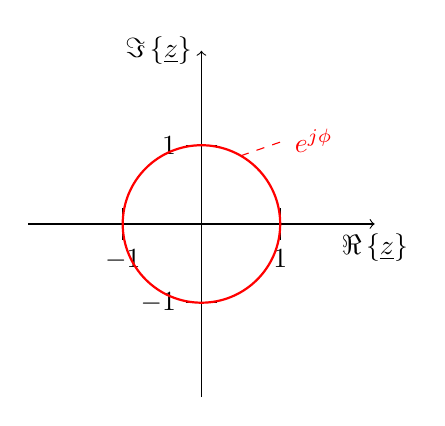
\begin{tikzpicture}
		\draw[->] (-2.2,0) -- (2.2,0) node[below, align=left]{$\Re\left\{\underline{z}\right\}$};
		\draw[->] (0,-2.2) -- (0,2.2) node[left, align=right]{$\Im\left\{\underline{z}\right\}$};
		%\draw (0:1) arc(0:360:1);
		\draw (1,0.2) -- (1,-0.2) node[below]{$1$};
		\draw (-1,0.2) -- (-1,-0.2) node[below]{$-1$};
		\draw (0.2,1) -- (-0.2,1) node[left]{$1$};
		\draw (0.2,-1) -- (-0.2,-1) node[left]{$-1$};
		
		\draw[thick, red] (0:1) arc(0:360:1);
		\draw[dashed, red] (60:1) -- (45:1.5) node[right, align=left, color=red]{$e^{j \phi}$};
	\end{tikzpicture}
	\caption{Complex plane of the complex frequency variable $\underline{z}$}
	\label{fig:ch04:ztrafo_z_cmplx_plane}
\end{figure}

In the \acf{DTFT}, $A = 1$ as a special case. The remainig $e^{j \phi}$ describes the unit circle in the complex plane. Like the Fourier transform, it assumes a steady-state, whereas the z-transform delivers a complete description of a time-discrete system. The z-transform is preferred for transient analysis of a time-discrete system. Its zeros $\underline{z}_0$ and poles $\underline{z}_\infty$ determine the stability of the system.

Figure \ref{fig:ch04:ztrafo_z_cmplx_plane} makes evident the $2 \pi$-periodicity of both the \ac{DTFT} and z-transform. The frequency $e^{j \phi}$ repeats every $2 \pi$.

\subsection{Discrete Fourier Transform}

\subsubsection{Periodic Sequences}

Given is an $N$-periodic sequence of samples $\underline{x}_p[n]$:
\begin{equation}
	\underline{x}_p[n] = \underline{x}_p[n + mN] \qquad \forall \; m \in \mathbb{Z}
\end{equation}

A corollary of the periodicity is that the \ac{DTFT} $\underline{X}_{2 \pi} \left(e^{j \phi}\right)$ or $\underline{X}_{\frac{2\pi}{T_S}} \left(e^{j T_S \omega}\right)$, respectively, is not only periodic. It is zero for
\begin{itemize}
	\item $\underline{X}_{2 \pi} \left(e^{j \phi}\right) = 0$ for $\phi \neq m \frac{2\pi}{N}$ where $m \in \mathbb{Z}$, or
	\item $\underline{X}_{\frac{2\pi}{T_S}} \left(e^{j T_S \omega}\right) = 0$ for $\omega \neq m \frac{2\pi}{T_S N}$ where $m \in \mathbb{Z}$.
\end{itemize}
The \ac{DTFT} itself becomes a series of pulses (Dirac comb) with an equidistant spacing of
\begin{itemize}
	\item $\frac{2\pi}{N}$ for $\underline{X}_{2 \pi} \left(e^{j \phi}\right)$, or
	\item $\frac{2\pi}{T_S N}$ for $\underline{X}_{\frac{2\pi}{T_S}} \left(e^{j T_S \omega}\right)$, respectively.
\end{itemize}

This can be explained using the duality of the \ac{DTFT}:
\begin{figure}[H]
	\centering
	\begin{adjustbox}{scale=0.75}
		\begin{tikzpicture}
			\node[align=center, minimum width=2.5cm, minimum height=1.5cm] (TD1) {Sampled data is a Dirac comb\\ $\underline{x}_S(t) = \sum\limits_{n = -\infty}^{\infty} \underline{x}[n] \delta\left(t - n T_S\right)$};
			\node[align=center, minimum width=2.5cm, minimum height=1.5cm, right=3.5cm of TD1] (TD2) {Sampled data is periodic\\ $\underline{x}_S(t) = \underline{x}_S(t + m N {T_S})$};
			\node[align=center, minimum width=2.5cm, minimum height=1.5cm, below=2cm of TD1] (FD1) {Spectrum is periodic\\ $\underline{X}_{\frac{2\pi}{T_S}}(e^{j T_S \omega}) = \underline{X}_{\frac{2\pi}{T_S}}(e^{j T_S \left(\omega + \omega_S\right)})$};
			\node[align=center, minimum width=2.5cm, minimum height=1.5cm, below=2cm of TD2] (FD2) {Spectrum is a Dirac comb\\ $\underline{X}_{\frac{2\pi}{T_S}}(e^{j T_S \omega}) = \frac{1}{N} \sum\limits_{n = -\infty}^{\infty} \underline{X}[k] \delta\left(\omega - \frac{k}{N} \omega_S\right)$};
			
			\node[align=right, anchor=east, left=3cm of TD1] (LabelTD) {\textbf{Time domain}};
			\node[align=right, anchor=east, below=2cm of LabelTD] (LabelFD) {\textbf{Frequency domain}};
			\node[align=right, above=1cm of TD1] (Func1) {\textbf{Non-periodic function}};
			\node[align=right, above=1cm of TD2] (Func2) {\textbf{Periodic function}};
			
			%\draw (TD1) node[midway, align=right, rotate=-90]{$\TransformHoriz$} (FD1);
			%\draw (TD2) node[midway, align=right, rotate=-90]{$\TransformHoriz$} (FD2);
			\draw[o-*, thick] (TD1.south) -- (FD1.north);
			\draw[o-*, thick] (TD2.south) -- (FD2.north);
			
			\draw[thick] (TD1.south east) -- (FD2.north west);
			\draw[thick] (TD2.south west) -- (FD1.north east);
		\end{tikzpicture}
	\end{adjustbox}
	\caption{Due to the duality, the \ac{DTFT} of a periodic signal is series of pulses (Dirac comb).}
\end{figure}

The \ac{DTFT} of a periodic signal is still periodic. The maximum number of unique, discrete frequency samples in the \ac{DTFT} is
\begin{equation}
	\frac{\text{Periodicity of the \ac{DTFT}}}{\text{Spacing between the pulses}} = \frac{\frac{2\pi}{T_S}}{\frac{2\pi}{T_S N}} = N
\end{equation}

Because of the periodicity of both the time-domain and frequency-domain signal, the signal is fully determined by either
\begin{itemize}
	\item $N$ samples in the time domain, or
	\item $N$ samples in the frequency domain.
\end{itemize}

The samples in the frequency domain are
\begin{equation}
	\underline{X}[k] = \left.\underline{X}_{2 \pi} \left(e^{j \phi}\right)\right|_{\phi = k \frac{2\pi}{N}} = \left.\underline{X}_{\frac{2\pi}{T_S}} \left(e^{j T_S \omega}\right)\right|_{\omega = k \frac{2\pi}{T_S N}} = \sum\limits_{n = 0}^{N-1} \underline{x}[n] e^{-j 2\pi \frac{k}{N} n}
\end{equation}
where $k \in \mathbb{Z}$ is the discrete frequency variable. The summation boundaries $[0, N-1]$ can be replaced by any sequence of length $N$, because $\underline{x}[n]$ is $N$-periodic.

$\underline{X}[k]$ is the \ac{DFT}. $\underline{X}[k]$ is $N$-periodic.

The \ac{DTFT} is obtained by:
\begin{equation}
	\underline{X}_{\frac{2\pi}{T_S}} \left(e^{j T_S \omega}\right) = \frac{2\pi}{N T_S} \sum\limits_{k = -\infty}^{\infty} \underline{X}[k] \cdot \delta\left(\omega - \frac{k}{N} \underbrace{\frac{2\pi}{T_S}}_{= \omega_S}\right)
\end{equation}

\textit{Remark:} $\omega$ is normalized to $\frac{N T_S}{2\pi}$. Accordingly, the sum is normalized to $\frac{2\pi}{N T_S}$. Considerations analogous to the explanation on page \pageref{ref:ch04:normalization_xs} apply.

The inverse \ac{DTFT} is:
\begin{equation}
	\begin{split}
		\underline{x}[n] &= \frac{T_S}{2 \pi} \int\limits_{- \frac{\pi}{T_S}}^{+ \frac{\pi}{T_S}} \frac{2\pi}{N T_S} \sum\limits_{k = -\infty}^{\infty} \underline{X}[k] \cdot \delta\left(\omega - \frac{k}{N} \frac{2\pi}{T_S}\right) \cdot e^{+ j \omega T_S n} \, \mathrm{d} \omega \\
		 &\qquad \text{Integration boundaries propagate to summation boundaries via $\omega - \frac{k}{N} \frac{2\pi}{T_S} \stackrel{!}{=} 0$:} \\
		 &= \frac{1}{N} \sum\limits_{k = -\frac{N}{2}}^{\frac{N}{2}} \underline{X}[k] \cdot \int\limits_{- \frac{\pi}{T_S}}^{+ \frac{\pi}{T_S}} \delta\left(\omega - \frac{k}{N} \frac{2\pi}{T_S}\right) \cdot e^{+ j \omega T_S n} \, \mathrm{d} \omega \\
		 &\qquad \text{Using the Dirac measure:} \\
		 &= \frac{1}{N} \sum\limits_{k = -\frac{N}{2}}^{\frac{N}{2}} \underline{X}[k] \cdot e^{+ j 2\pi \frac{k}{N} n}
	\end{split}
\end{equation}
This is the inverse \ac{DFT}. Again the summation boundaries of $[-\frac{N}{2}, \frac{N}{2}]$ can be replaced by any sequence of length $N$, because $\underline{X}[k]$ is $N$-periodic.

\begin{definition}{Discrete Fourier transform}
	The \index{discrete Fourier transform} \textbf{\acf{DFT}} of a $N$-periodic sequence $\underline{x}[n]$ is:
	\begin{equation}
		\underline{X}[k] = \mathcal{F}_{\text{DFT}}\left\{\underline{x}[n]\right\} = \sum\limits_{n \in N} \underline{x}[n] \cdot e^{-j 2\pi \frac{k}{N} n}
		\label{eq:ch04:dft}
	\end{equation}
	
	The \index{inverse discrete Fourier transform} \textbf{inverse discrete Fourier transform} is:
	\begin{equation}
		\underline{x}[n] = \mathcal{F}_{\text{DFT}}^{-1}\left\{\underline{X}[k]\right\} = \frac{1}{N} \sum\limits_{k \in N} \underline{X}[k] \cdot e^{+ j 2\pi \frac{k}{N} n}
		\label{eq:ch04:idft}
	\end{equation}
	
	Both $\underline{X}[k]$ and $\underline{x}[n]$ are $N$-periodic. The summation boundaries can be chosen to any sequence of length $N$.
\end{definition}

\subsubsection{Properties}

The \ac{DFT} is derived from the \ac{DTFT} and \ac{CTFT}. Therefore, all properties apply likewise.
\begin{itemize}
	\item Linearity
	\item Time shift, frequency shift
	\item Convolution theorem
	\item Duality
	\item Symmetry rules
\end{itemize}

\subsection{Orthogonality of the \acs{DFT} Frequency Vectors}

Both the time-domain sequence $\underline{x}[n]$ and frequency-domain sequence $\underline{X}[k]$ can be interpreted as vectors:
\begin{itemize}
	\item $\cmplxvect{x} = \left[\underline{x}[0], \underline{x}[1], \dots, \underline{x}[N-1]\right]^{\mathrm{T}}$
	\item $\cmplxvect{X} = \left[\underline{X}[0], \underline{X}[1], \dots, \underline{X}[N-1]\right]^{\mathrm{T}}$
\end{itemize}

The \ac{DFT} \eqref{eq:ch04:dft} can be expressed as a linear system of equation:
\begin{equation}
	\cmplxvect{X} = \underline{\mat{F}} \cdot \cmplxvect{x}
\end{equation}

The $N \times N$ transformation matrix $\underline{\mat{F}}$ is the \index{DFT matrx} \textbf{\ac{DFT} matrix} with the elements:
\begin{equation}
	\underline{F}_{pq} = \underline{w}^{p \cdot q}
\end{equation}
where $\underline{w}$ is the $N$-th \index{primitive root of unity} \textbf{primitive root of unity}\footnote{The primitive root of unity divide the unit circle $e^{j \phi}$ into equally sized segments.}.
\begin{equation}
	\underline{w} = e^{j \frac{2 \pi}{N}}
\end{equation}
So
\begin{equation}
	\underline{\mat{F}} = \left[
	\begin{matrix}
		1 & 1 & 1 & 1 & \ldots & 1 \\
		1 & \underline{w} & \underline{w}^2 & \underline{w}^3 & \ldots & \underline{w}^{N-1} \\
		1 & \underline{w}^2 & \underline{w}^4 & \underline{w}^6 & \ldots & \underline{w}^{2\left(N-1\right)} \\
		1 & \underline{w}^3 & \underline{w}^6 & \underline{w}^9 & \ldots & \underline{w}^{3\left(N-1\right)} \\
		\vdots & \vdots & \vdots & \vdots & \ddots & \vdots \\
		1 & \underline{w}^{N-1} & \underline{w}^{2\left(N-1\right)} & \underline{w}^{3\left(N-1\right)} & \ldots & \underline{w}^{\left(N-1\right)\left(N-1\right)} \\
	\end{matrix}
	\right]
\end{equation}

The inverse \ac{DFT} is, using the conjugate complex $\overline{\underline{\mat{F}}}$:
\begin{equation}
	\cmplxvect{x} = \frac{1}{N} \overline{\underline{\mat{F}}} \cdot \cmplxvect{X}
\end{equation}

Each row and column of $\underline{\mat{F}}$ is a vector of powers of the $N$-th primitive root of unity $\underline{w}$. A row with the index $k$ is $\cmplxvect{u}_k$.
\begin{equation}
	\begin{split}
		\cmplxvect{u}_k &= \left[\left.\underline{w}^{k \cdot q}\right| q = 0, 1, \dots, N-1\right]^{\mathrm{T}} \\
		 &= \left[1, \underline{w}^{k}, \underline{w}^{2 k}, \underline{w}^{3 k}, \dots, \underline{w}^{k \left(N-1\right)} \right]^{\mathrm{T}} \\
		 &= \left[1, e^{j \frac{2 \pi}{N} k}, e^{j \frac{2 \pi}{N} 2 k}, e^{j \frac{2 \pi}{N} 3 k}, \dots, e^{j \frac{2 \pi}{N} k \left(N-1\right)} \right]^{\mathrm{T}} \\
	\end{split}
\end{equation}
Each vector $\cmplxvect{u}_k$ is the basis for the associated frequency sample $\underline{X}[k]$.

It can be shown that the vectors $\cmplxvect{u}_k$ are orthogonal. They form an \index{orthogonal basis} \textbf{orthogonal basis}. This can be proven by their inner product:
\begin{equation}
	\begin{split}
		\langle \cmplxvect{u}_p, \overline{\cmplxvect{u}_q} \rangle &= \sum\limits_{n=0}^{N-1} \left(e^{j \frac{2 \pi}{N} p n}\right) \overline{\left(e^{j \frac{2 \pi}{N} q n}\right)} \\
		 &= \sum\limits_{n=0}^{N-1} e^{j \frac{2 \pi}{N} \left(p - q\right) n} \\
		 &= N \delta_{pq}
	\end{split}
\end{equation}

\textit{Remark:} $\delta_{pq}$ is the Kronecker delta here.

\begin{itemize}
	\item The vectors $\cmplxvect{u}_p$ and $\cmplxvect{u}_q$ are orthogonal ($\delta_{pq} = 0$) for $p \neq q$.
	\item $\delta_{pq}$ is non-zero only if $p = q$.
\end{itemize}

\begin{fact}
	The basis of the frequency samples of a \ac{DFT} are orthogonal.
\end{fact}

\subsection{Processing of Non-Periodic Signals}

In practical digital systems, signals are non-periodic. A non-periodic sequence $\underline{x}[n]$ can be fully transformed by the \ac{DTFT}.
\begin{equation}
	\underline{x}[n] \TransformHoriz \mathcal{F}_{\text{DTFT}}\left\{\underline{x}[n]\right\} = \underline{X}_{\frac{2\pi}{T_S}}\left(e^{j T_S \omega}\right)
\end{equation}

However, it is not feasible to implement a \ac{DTFT}, because the sums and integrals run over an indefinite interval. Therefore, the transforms are approximated by the \ac{DFT}.

\subsubsection{Windowing and Periodic Continuation}

A sequence of length $N$ is taken out of $\underline{x}[n]$:
\begin{equation}
	\underline{\tilde{x}}_N[n] = \left[\underline{x}[m], \underline{x}[m+1], \underline{x}[m+1], \dots, \underline{x}[m+N-1]\right]
\end{equation}
The act of extracting $N$ subsequent samples out of $\underline{x}[n]$ is called \index{windowing} \textbf{windowing}. To illustrate this, imagine that you watch a sequence moving to the left through a window. The movement to the left is the time advance. Because of the window, you see a certain extract of $\underline{x}[n]$ only at one time.

%TODO
%\todo{Window illustration}

This sequence is repeated indefinitely (\emph{periodic continuation}):
\begin{equation}
	\underline{x}_N[n] = \underline{\tilde{x}}_N[n \mod N]
\end{equation}
Thus, $\underline{x}_N[n]$ is periodic:
\begin{equation}
	\underline{x}_N[n] = \underline{x}_N[n + q N] \qquad \forall \; q \in \mathbb{Z}
\end{equation}

Now, $\underline{x}_N[n]$ can be transformed to the frequency-domain using the \ac{DFT}.
\begin{equation}
	\underline{x}_N[n] \TransformHoriz \mathcal{F}_{\text{DFT}}\left\{\underline{x}[n]\right\} = \underline{X}[k]
\end{equation}

The periodic continuation is just a theoretical explanation. In practise, it is enough to calculate the \ac{DFT} over $N$ subsequent samples out of $\underline{x}[n]$.
\begin{equation}
	\begin{split}
		\underline{X}_{\frac{2\pi}{T_S}}\left(e^{j T_S \omega}\right) &\approx \begin{cases}
			\left.\underline{X}[k]\right|_{k = N \frac{T_S}{2\pi} \omega} & \quad \text{if } \left(N \frac{T_S}{2\pi} \omega\right) \in \mathbb{Z}, \\
			0 & \quad \text{if } \left(N \frac{T_S}{2\pi} \omega\right) \notin \mathbb{Z}.
		\end{cases} \\
		\underline{X}_{\frac{2\pi}{T_S}}\left(e^{j 2 \pi \frac{k}{N}}\right) &\approx \underline{X}[k] = \sum\limits_{n=0}^{N-1} \underline{x}_N[n] e^{-j 2 \pi \frac{k}{N} n}
	\end{split}
	\label{eq:ch04:dtft_sampling}
\end{equation}

Windowing and periodic continuation is, in fact, a sampling of the \ac{DTFT} (see \eqref{eq:ch04:dtft_sampling}).

\subsubsection{Window Functions}

The widowing of $\underline{x}[n]$ to obtain $\underline{x}_N[n]$ as discussed before did not change the values of $\underline{x}[n]$. This can be expressed as a multiplication of the original sequence with the rectangular function:
\begin{equation}
	\underline{x}_W[n] = \underline{x}_N[n] \cdot \underbrace{w_{rect,M}[n]}_{\text{Rectangular window}}
\end{equation}
where $w_{rect,M}[n]$ is the rectangular function of the length $M$:
\begin{equation}
	w_{rect,M}[n] = \begin{cases}
		1 &\quad \text{if } \; -\frac{M-1}{2} \leq n \leq \frac{M-1}{2}, \\
		0 &\quad \text{else}.
	\end{cases}
\end{equation}
$M$ shall be an odd number.

$w_M[n]$ is called \index{window function} \textbf{window function}.
\begin{definition}{Window function}
	A \index{window function} \textbf{window function} $w_M[n]$ is applied to the periodically continued sequence $\underline{x}_N[n]$ by multiplication:
	\begin{equation}
		\underline{x}_N[n] \equiv \underline{x}[n] \cdot w_M[n]
	\end{equation}
	
	Window functions are $w_M[n]$:
	\begin{itemize}
		\item limited to a length of $M$
		\item where $M$ is an odd number,
		\item always symmetric (even functions), and
		\item real-valued.
	\end{itemize}
\end{definition}

\subsubsection{Spectral Leakage}

In the frequency-domain, the multiplication becomes a convolution:
\begin{equation}
	\begin{split}
		\underline{X}_W[k] &= \mathcal{F}_{\text{DFT}}\left\{\underline{x}_W[n]\right\} \\
		 &= \mathcal{F}_{\text{DFT}}\left\{\underline{x}_N[n] \cdot w[n]\right\} \\
		 &= \underline{X}_N[k] * \underline{W}[k] \\
		 &= \sum\limits_{l=0}^{N-1} \underline{X}_N[l] * \underline{W}[k-l]
	\end{split}
\end{equation}

This has some implications:
\begin{itemize}
	\item Each frequency component in $\underline{X}_N[k]$ creates frequency components in \underline{all} $\underline{X}_W[k]$.
	\item A mono-chromatic signal, which would be non-zero at only one $k$ and zero everywhere else, has non-zero components everywhere in $\underline{X}_W[k]$.
	\item The non-zero frequency components produced by the convolution show up as noise and \underline{decrease the \ac{SNR}}.
\end{itemize}
This effect is called \index{spectral leakage} \textbf{spectral leakage}.

\begin{fact}
	The window changes only the amplitude spectrum, but not the phase of the sampled signal.
\end{fact}
\begin{itemize}
	\item The window function is an even, real-valued function.
	\item Its Fourier transform is therefore always real-valued, too.
	\item The purely real-valued ($\arg{\cdot} = 0 \text{ or } \pm \pi$) Fourier transform cannot change the phase of the signal.
\end{itemize}


\begin{figure}[H]
	\centering
	
	\subfloat[Original analogue signal]{
		\centering
		\begin{tikzpicture}
			\begin{axis}[
				height={0.15\textheight},
				width=0.35\linewidth,
				scale only axis,
				xlabel={$t$},
				ylabel={$x(t)$},
				%grid style={line width=.6pt, color=lightgray},
				%grid=both,
				grid=none,
				legend pos=north east,
				axis y line=middle,
				axis x line=middle,
				every axis x label/.style={
					at={(ticklabel* cs:1.05)},
					anchor=north,
				},
				every axis y label/.style={
					at={(ticklabel* cs:1.05)},
					anchor=east,
				},
				xmin=0,
				xmax=4.5,
				ymin=-1.2,
				ymax=1.2,
				%xtick={-1, -0.5, 0, 0.5, 1},
				%xticklabels={$- \omega_S$, $- \frac{\omega_S}{2}$, $0$, $\frac{\omega_S}{2}$, $\omega_S$},
				%ytick={0},
			]
				\addplot[red, thick, smooth, domain=0:4, samples=50] plot(\x, {cos(deg(pi*\x))});
				
				\pgfplotsinvokeforeach{0,0.25,...,4}{
					\addplot[blue] coordinates {(#1,0) (#1,{cos(deg(pi*#1))})};
					\addplot[blue, only marks, mark=o] coordinates {(#1,{cos(deg(pi*#1))})};
				}
			\end{axis}
		\end{tikzpicture}
	}
	\hfill
	\subfloat[Window function in the time-domain]{
		\centering
		\begin{tikzpicture}
			\begin{axis}[
				height={0.15\textheight},
				width=0.35\linewidth,
				scale only axis,
				xlabel={$n$},
				ylabel={$w_9[n]$},
				%grid style={line width=.6pt, color=lightgray},
				%grid=both,
				grid=none,
				legend pos=north east,
				axis y line=middle,
				axis x line=middle,
				every axis x label/.style={
					at={(ticklabel* cs:1.05)},
					anchor=north,
				},
				every axis y label/.style={
					at={(ticklabel* cs:1.05)},
					anchor=east,
				},
				xmin=-8.5,
				xmax=8.5,
				ymin=0,
				ymax=1.2,
				%xtick={-1, -0.5, 0, 0.5, 1},
				%xticklabels={$- \omega_S$, $- \frac{\omega_S}{2}$, $0$, $\frac{\omega_S}{2}$, $\omega_S$},
				%ytick={0},
			]
				\pgfplotsinvokeforeach{-4,-3,...,4}{
					\addplot[blue] coordinates {(#1,0) (#1,1)};
					\addplot[blue, only marks, mark=o] coordinates {(#1,1)};
				}
				\pgfplotsinvokeforeach{-8,-7,...,-5}{
					\addplot[blue, only marks, mark=o] coordinates {(#1,0)};
				}
				\pgfplotsinvokeforeach{5,6,...,8}{
					\addplot[blue, only marks, mark=o] coordinates {(#1,0)};
				}
			
%				\addplot[blue, thick] coordinates {(-0.5,0) (0,0)};
%				\addplot[blue, thick] coordinates {(0,1) (8,1)};
%				\addplot[blue, thick] coordinates {(8,0) (8.5,0)};
%				
%				\addplot[blue, thick, dashed] coordinates {(0,0) (0,1)};
%				\addplot[blue, thick, dashed] coordinates {(8,1) (8,0)};
			\end{axis}
		\end{tikzpicture}
	}

	\subfloat[Amplitude spectrum of the periodically continued signal]{ %  $\underline{X}_N[k]$
		\centering
		\begin{tikzpicture}
			\begin{axis}[
				height={0.15\textheight},
				width=0.35\linewidth,
				scale only axis,
				xlabel={$k$},
				ylabel={$\underline{X}_N[k]$},
				%grid style={line width=.6pt, color=lightgray},
				%grid=both,
				grid=none,
				legend pos=north east,
				axis y line=middle,
				axis x line=middle,
				every axis x label/.style={
					at={(ticklabel* cs:1.05)},
					anchor=north,
				},
				every axis y label/.style={
					at={(ticklabel* cs:1.05)},
					anchor=east,
				},
				xmin=-8.5,
				xmax=8.5,
				ymin=0,
				ymax=1.2,
				%xtick={-1, -0.5, 0, 0.5, 1},
				%xticklabels={$- \omega_S$, $- \frac{\omega_S}{2}$, $0$, $\frac{\omega_S}{2}$, $\omega_S$},
				%ytick={0},
			]
				\addplot[red] coordinates {(2,0) (2,1)};
				\addplot[red] coordinates {(-2,0) (-2,1)};
				\addplot[red, only marks, mark=o] coordinates {(-2,1) (2,1)};
				\pgfplotsinvokeforeach{-8,-7,...,-3}{
					\addplot[red, only marks, mark=o] coordinates {(#1,0)};
				}
				\pgfplotsinvokeforeach{-1,0,1}{
					\addplot[red, only marks, mark=o] coordinates {(#1,0)};
				}
				\pgfplotsinvokeforeach{3,4,...,8}{
					\addplot[red, only marks, mark=o] coordinates {(#1,0)};
				}
			\end{axis}
		\end{tikzpicture}
	}
	\hfill
	\subfloat[Amplitude spectrum of the window]{
		\centering
		\begin{tikzpicture}
			\begin{axis}[
				height={0.15\textheight},
				width=0.35\linewidth,
				scale only axis,
				xlabel={$k$},
				ylabel={$\underline{W}[k]$},
				%grid style={line width=.6pt, color=lightgray},
				%grid=both,
				grid=none,
				legend pos=north east,
				axis y line=middle,
				axis x line=middle,
				every axis x label/.style={
					at={(ticklabel* cs:1.05)},
					anchor=north,
				},
				every axis y label/.style={
					at={(ticklabel* cs:1.05)},
					anchor=east,
				},
				xmin=-8.5,
				xmax=8.5,
				ymin=0,
				ymax=9.5,
				%xtick={-1, -0.5, 0, 0.5, 1},
				%xticklabels={$- \omega_S$, $- \frac{\omega_S}{2}$, $0$, $\frac{\omega_S}{2}$, $\omega_S$},
				%ytick={0},
			]
				\addplot[blue, dashed, smooth, domain=-8:8, samples=50] plot(\x, {9*abs(asinc((pi*\x/8), 9))});
				\pgfplotsinvokeforeach{-8,-7,...,8}{
					\addplot[red] coordinates {(#1,0) (#1,{9*abs(asinc((pi*#1/8), 9))})};
					\addplot[red, only marks, mark=o] coordinates {(#1,{9*abs(asinc((pi*#1/8), 9))})};
				}
			
				\draw[blue, dashed] (axis cs:1.5,7) -- (axis cs:2.5,7) node[right,align=left,color=blue]{$\underline{W}\left(e^{j\phi}\right)$\\ $\phi=2\pi\frac{k}{N}$};
				\draw (axis cs:-1,7) node[left,align=right,color=blue]{Main lobe};
				\draw (axis cs:-2,3) node[left,align=right,color=blue]{Side lobes};
			\end{axis}
		\end{tikzpicture}
	}


	\subfloat[Amplitude spectrum of the windowed signal, showing spectral leakage]{
		\centering
		\begin{tikzpicture}
			\begin{axis}[
				height={0.15\textheight},
				width=0.7\linewidth,
				scale only axis,
				xlabel={$k$},
				ylabel={$\underline{X}_W[k]$},
				%grid style={line width=.6pt, color=lightgray},
				%grid=both,
				grid=none,
				legend pos=north east,
				axis y line=middle,
				axis x line=middle,
				every axis x label/.style={
					at={(ticklabel* cs:1.05)},
					anchor=north,
				},
				every axis y label/.style={
					at={(ticklabel* cs:1.05)},
					anchor=east,
				},
				xmin=-8.5,
				xmax=8.5,
				ymin=0,
				ymax=12.5,
				%xtick={-1, -0.5, 0, 0.5, 1},
				%xticklabels={$- \omega_S$, $- \frac{\omega_S}{2}$, $0$, $\frac{\omega_S}{2}$, $\omega_S$},
				%ytick={0},
			]
				\addplot[blue, dashed, smooth, domain=-8:8, samples=50] plot(\x, {9*abs(asinc((pi*(\x+2)/8), 9)) + 9*abs(asinc((pi*(\x-2)/8), 9))});
				\pgfplotsinvokeforeach{-8,-7,...,8}{
					\addplot[red] coordinates {(#1,0) (#1,{9*abs(asinc((pi*(#1+2)/8), 9)) + 9*abs(asinc((pi*(#1-2)/8), 9))})};
					\addplot[red, only marks, mark=o] coordinates {(#1,{9*abs(asinc((pi*(#1+2)/8), 9)) + 9*abs(asinc((pi*(#1-2)/8), 9))})};
				}
				\draw[blue, dashed] (axis cs:3,9) -- (axis cs:3.7,9) node[right,align=left,color=blue]{$\left.\underline{X}_W\left(e^{j\phi}\right)\right|_{\phi=2\pi\frac{k}{N}}$};
			\end{axis}
		\end{tikzpicture}
	}

	\caption{Spectral leakage of a mono-chromatic signal}
\end{figure}

In the above example:
\begin{itemize}
	\item The monochromatic signal has two ideal pulses in its amplitude spectrum.
	\item The rectangular window has a sinc-like amplitude spectrum.
	\item Due to the convolution, the ideal pulses of the monochromatic signal are ``leak'' across the frequency axis and take a sinc-like pattern, too.
\end{itemize}

The selection of the window function has implications on the spectral leakage:
\begin{itemize}
	\item The width of the \emph{main lobe}, defines how much the sampled signal is spread across the frequency axis.
	\item The \emph{main lobe} should be narrow, in order to retain the original shape of the signal.
	\item The amplitudes of the \emph{side lobes} define the noise, which emerges.
	\item The \emph{side lobes} should be as weak as possible regarding their amplitudes, in order to reduce the noise and improve the \ac{SNR}.
\end{itemize}

\begin{fact}
	Generally, window functions with narrow main lobes have strong side lobes, and vice versa. So, there is always a trade-off.
\end{fact}

\begin{landscape}
	\subsubsection{Some Window Functions}
	
	\begin{longtable}[H]{|l|l|l|l|l|}
		\hline
		Name & Function $w[n]$ & Peak side lobe & Main lobe width & Time domain and frequency response \\
		\hline
		\hline
		Rectangular & $w[n] = \begin{cases}1, &\quad 0 \leq n \leq M,\\ 0, &\quad \text{otherwise}.\end{cases}$ & \SI{-13}{dB} & $\frac{4\pi}{M+1}$ & \includegraphics[width=5cm]{svg/ch04_win_rect.pdf} \\
		\hline
		Hamming & $w[n] = \begin{cases}0.54 - 0.46 \cos\left(\frac{2 \pi n}{M}\right), &\quad 0 \leq n \leq M,\\ 0, &\quad \text{otherwise}.\end{cases}$ & \SI{-41}{dB} & $\frac{8\pi}{M}$ &  \includegraphics[width=5cm]{svg/ch04_win_hamming.pdf} \\
		\hline
		Hann & $w[n] = \begin{cases}0.5 - 0.5 \cos\left(\frac{2 \pi n}{M}\right), &\quad 0 \leq n \leq M,\\ 0, &\quad \text{otherwise}.\end{cases}$ & \SI{-31}{dB} & $\frac{8\pi}{M}$ &  \includegraphics[width=5cm]{svg/ch04_win_hann.pdf} \\
		\hline
		Blackman & $w[n] = \begin{cases}0.42 - 0.5 \cos\left(\frac{2 \pi n}{M}\right) & \\ \quad + 0.08 \cos\left(\frac{4 \pi n}{M}\right), &\quad 0 \leq n \leq M,\\ 0, &\quad \text{otherwise}.\end{cases}$ & \SI{-57}{dB} & $\frac{12\pi}{M}$ &  \includegraphics[width=5cm]{svg/ch04_win_blackman.pdf} \\
		\hline
		Bartlett & $w[n] = \begin{cases}2n/M, &\quad 0 \leq n \leq M/2,\\ 2 - 2n/M, &\quad M/2 < n \leq M,\\ 0, &\quad \text{otherwise}.\end{cases}$ & \SI{-25}{dB} & $\frac{8\pi}{M}$ &  \includegraphics[width=5cm]{svg/ch04_win_tri.pdf} \\
		\hline
		Gauss & $w[n] = \begin{cases}\exp\left(- \frac{1}{2} \left(\frac{n - M/2}{\sigma M / 2}\right)^2\right), &\quad 0 \leq n \leq M,\\ 0, &\quad \text{otherwise}.\end{cases}$ & \multicolumn{2}{l|}{Adjustable by $\sigma$} &  \includegraphics[width=5cm]{svg/ch04_win_gauss.pdf} \\
		\hline
	\end{longtable}

	\textit{Picture credits:} \licensequote{\cite{Niemitalo2013}}{Olli Niemitalo}{\href{https://creativecommons.org/publicdomain/zero/1.0/deed.en}{CC0 1.0}}
	
	\begin{itemize}
		\item Now, you see the trade-off which must be made between narrow main lobe and weak side lobes.
		\item The rectangular window has a narrow main lobe but strong side lobes.
		\item The Blackman window has weak side lobes but a wide main lobe.
	\end{itemize}
\end{landscape}


\section{Analogies Of Time-Continuous and Time-Discrete Signals and Systems}

All relations shown here are analogous to the \ac{CTFT}. Their deduction is analogous to Chapters 2 and 3.

\subsection{Transforms}

\begin{table}[H]
	\centering
	\begin{tabular}{|p{0.3\linewidth}||p{0.3\linewidth}|p{0.3\linewidth}|}
		\hline
		{} & \textbf{Frequency-Continuous Domain} & \textbf{Frequency-Discrete Domain} \\
		\hline
		\hline
		\textbf{Time-Continuous Domain} & Fourier transform & Fourier series \\
		\hline
		\textbf{Time-Discrete Domain} & Discrete-Time Fourier transform & Discrete Fourier transform \\
		\hline
	\end{tabular}
\end{table}

\subsubsection{Obtaining a frequency-continuous domain:}

\begin{minipage}{0.45\linewidth}
	\textbf{From the time-continuous domain (analog signal):}
	
	\vspace{0.5em}
	
	\acf{CTFT}:
	\begin{equation*}
		\underline{X}(j \omega) = \int\limits_{t = -\infty}^{\infty} \underline{x}(t) \cdot e^{-j \omega t} \, \mathrm{d} t
	\end{equation*}
	
	Inverse Fourier transform:
	\begin{equation*}
		\underline{x}(t) = \frac{1}{2 \pi} \int\limits_{\omega = -\infty}^{\infty} \underline{X}(j \omega) \cdot e^{+ j \omega t} \, \mathrm{d} \omega
	\end{equation*}
	
	\begin{itemize}
		\item Continuous time: $t \in \mathbb{R}$
		\item Continuous frequency: $\omega \in \mathbb{R}$
	\end{itemize}
\end{minipage}
\hfill
\begin{minipage}{0.45\linewidth}
	\textbf{From the time-discrete domain (digital signal):}
	
	\vspace{0.5em}
	
	\acf{DTFT}:
	\begin{equation*}
		\underline{X}_{2\pi}(e^{j \phi}) = \sum\limits_{n = -\infty}^{\infty} \underline{x}[n] \cdot e^{- j \phi n}
	\end{equation*}
	
	Inverse discrete-time Fourier transform:
	\begin{equation*}
		\underline{x}[n] = \frac{1}{2 \pi} \int\limits_{- \pi}^{+ \pi} \underline{X}_{2\pi}(e^{j \phi}) \cdot e^{+ j \phi n} \, \mathrm{d} \phi
	\end{equation*}
	
	\begin{itemize}
		\item Discrete time: $n \in \mathbb{Z}$
		\item Continuous frequency: $\phi \in \mathbb{R}$
	\end{itemize}
\end{minipage}

\subsubsection{Obtaining a frequency-discrete domain:}

\begin{minipage}{0.45\linewidth}
	\textbf{From the time-continuous domain (analog signal):}
	
	\vspace{0.5em}
	
	Fourier analysis:
	\begin{equation*}
		\underline{X}[k] = \frac{\omega_0}{2 \pi} \int\limits_{-\frac{T_0}{2}}^{\frac{T_0}{2}} \underline{x}(t) \cdot e^{-j k \omega_0 t} \, \mathrm{d} t
	\end{equation*}
	
	Fourier series:
	\begin{equation*}
		\underline{x}(t) = \sum\limits_{k = -\infty}^{\infty} \underline{X}[k] \cdot e^{+ j k \omega_0 t}
	\end{equation*}
	
	\begin{itemize}
		\item Continuous time: $t \in \mathbb{R}$
		\item Discrete frequency: $k \in \mathbb{Z}$
	\end{itemize}
\end{minipage}
\hfill
\begin{minipage}{0.45\linewidth}
	\textbf{From the time-discrete domain (digital signal):}
	
	\vspace{0.5em}
	
	\acf{DFT}:
	\begin{equation*}
		\underline{X}[k] = \sum\limits_{n = 0}^{N - 1} \underline{x}[n] \cdot e^{- j \frac{2 \pi}{N} k n}
	\end{equation*}
	
	Inverse discrete Fourier transform:
	\begin{equation*}
		\underline{x}[n] = \frac{1}{N} \sum\limits_{k = 0}^{N - 1} \underline{X}[k]  \cdot e^{+ j \frac{2 \pi}{N} k n}
	\end{equation*}
	
	\begin{itemize}
		\item Discrete time: $n \in \mathbb{Z}$
		\item Discrete frequency: $k \in \mathbb{Z}$
	\end{itemize}
\end{minipage}

\subsubsection{Properties of the \acs{DFT}}

\begin{itemize}
	\item Linearity:
	\begin{equation}
		\mathcal{F}_{\text{DFT}}\left\{a \underline{x}[n] + b \underline{y}[n]\right\} = a \mathcal{F}_{\text{DFT}}\left\{\underline{x}[n]\right\} + b \mathcal{F}_{\text{DFT}}\left\{\underline{y}[n]\right\}
	\end{equation}
	\item Time shift:
	\begin{equation}
		\mathcal{F}_{\text{DFT}}\left\{\underline{x}[n - m]\right\}[k] = \underline{X}[k] \cdot e^{-j 2 \pi \frac{k}{N} m}
	\end{equation}
	\item Frequency shift:
	\begin{equation}
		\mathcal{F}_{\text{DFT}}\left\{\underline{x}[n] \cdot e^{-j 2 \pi \frac{n}{N} m}\right\}[k] = \underline{X}[k-m]
	\end{equation}
	\item Multiplication in the time-domain becomes convolution in the frequency domain:
	\begin{equation}
		\mathcal{F}_{\text{DFT}}\left\{\underline{x}[n] \cdot \underline{y}[n]\right\}[k] = \underline{X}[k] * \underline{Y}[k] = \sum_{l=0}^{N} \underline{X}[l] \underline{Y}[(k - l) \mod N]
	\end{equation}
	\item Convolution in the time-domain becomes multiplication in the frequency domain:
	\begin{equation}
		\mathcal{F}_{\text{DFT}}\left\{\underline{x}[n] * \underline{y}[n]\right\}[k] = \mathcal{F}_{\text{DFT}}\left\{\sum_{l=0}^{N} \underline{x}[l] \underline{y}[(n - l) \mod N]\right\}[k] = \underline{X}[k] \cdot \underline{Y}[k]
	\end{equation}
	\item Duality:
	\begin{equation}
		\mathcal{F}_{\text{DFT}}\left\{\underline{X}[n]\right\}[k] = N \cdot \underline{x}[N - k]
	\end{equation}
	where $\underline{x} \TransformHoriz \underline{X}$.
	\item Symmetry for real-valued $\underline{x}[n]$:
	\begin{equation}
		\underline{X}[k] = \overline{\underline{X}[N-k]} \qquad \forall \; \underline{x}[n] \in \mathbb{R}
	\end{equation}
\end{itemize}

%\subsubsection{Spectrum}

\subsection{Systems}

\textit{Remark:} In contrast to signals, systems are analysed using the z-transform (general form of the \ac{DTFT}). For signals, the \ac{DFT} is preferred.

\begin{figure}[H]
	\centering
	\begin{tikzpicture}
		\node[draw, block] (System) {System\\ $\underline{h}[n]$};
		\draw[<-o] (System.west) -- ++(-2cm, 0) node[above, align=center]{Input signal\\ $\underline{x}[n]$};
		\draw[->] (System.east) -- ++(2cm, 0) node[above, align=center]{Output signal\\ $\underline{y}[n]$};
	\end{tikzpicture}
	\caption{A time-discrete system with input and output}
\end{figure}

A time-discrete system is characterized by either
\begin{itemize}
	\item its \index{transfer function} transfer function
	\begin{equation}
		\underline{H}(\underline{z}) = \frac{\underline{Y}(\underline{z})}{\underline{X}(\underline{z})}
	\end{equation}
	or
	\item its impulse response.
	\begin{equation}
		\underline{h}[n] = \mathcal{Z}^{-1}\left\{\underline{H}(\underline{z})\right\}
	\end{equation}
\end{itemize}

In the time domain, the output is a convolution of the input and the impulse response.
\begin{equation}
	\underline{y}[n] = \underline{h}[n] * \underline{x}[n] = \sum\limits_{l = -\infty}^{\infty} \underline{h}[l] \underline{x}[n-l]
\end{equation}

The systems output is the impulse response $\underline{y}[n] = \underline{h}[n]$ if the input is a Kronecker delta function $\underline{x}[n] = \delta[n]$.
\begin{equation}
	\underline{h}[n] * \delta[n] = \underline{h}[n]
\end{equation}
Or in the frequency domain
\begin{equation}
	\underline{H}(\underline{z}) \cdot \underbrace{\mathcal{Z}\left\{\delta[n]\right\}}_{= 1} = \underline{H}(\underline{z})
\end{equation}

\begin{excursus}{Kronecker delta}
	The \index{Kronecker delta} Kronecker delta $\delta[n]$ equivalent of the Dirac delta function $\delta(t)$ in the discrete domain.
	
	\begin{equation*}
		\delta(t) = \begin{cases}
			\infty & \quad \text{if } t = 0, \\
			0 & \quad \text{if } t \neq 0.
		\end{cases}
	\end{equation*}
	
	\begin{equation*}
		\delta[n] = \begin{cases}
			1 & \quad \text{if } n = 0, \\
			0 & \quad \text{if } n \neq 0.
		\end{cases}
	\end{equation*}
	
	The Dirac delta function $\delta(t)$ is an indefinitely narrow pulse but indefinitely high. In contrast to that, the Kronecker delta $\delta[n]$ is of unity length and unity height. Both functions sum up to $1$.
	\begin{equation}
		\int\limits_{-\infty}^{\infty} \delta(t) \, \mathrm{d} t = \sum\limits_{n = -\infty}^{\infty} \delta[n] = 1
	\end{equation}
\end{excursus}

\subsection{Spectral Density}

\subsubsection{Cross-Correlation and Autocorrelation}

All considerations apply for ergodic or \ac{WSS} processes only:

\begin{itemize}
	\item Cross-correlation:
	\begin{equation}
		\underline{\mathrm{R}}_{xy}[n] = \left(\underline{x} \star \underline{y}\right)[n] = \sum\limits_{m=0}^{N-1} \underline{x}[m] \overline{\underline{y}[(m+n) \mod N]}
	\end{equation}
	\item Autocorrelation:
	\begin{equation}
		\underline{\mathrm{R}}_{xx}[n] = \left(\underline{x} \star \underline{x}\right)[n] = \sum\limits_{m=0}^{N-1} \underline{x}[m] \overline{\underline{x}[m+n]}
	\end{equation}
\end{itemize}

\subsubsection{Energy Spectral Density}

Parseval's theorem for discrete systems:
\begin{equation}
	\sum\limits_{n=0}^{N-1} \left|\underline{x}[n]\right|^2 = \frac{1}{N} \sum\limits_{k=0}^{N-1} \left|\underline{X}[k]\right|^2
\end{equation}

The signal energy is defined to:
\begin{equation}
	E = T_S^2 \sum\limits_{n=0}^{N-1} \left|\underline{x}[n]\right|^2 \stackrel{!}{=} \sum\limits_{n=0}^{N-1} \underline{\mathrm{S}}_{E,xx}[k]
\end{equation}
The sampling period $T_S$ (spacing between the samples) must be kept, because the physical energy depends on the duration of the samples.

The energy spectral density is:
\begin{equation}
	\underline{\mathrm{S}}_{E,xx}[k] = \frac{T_S^2}{N} \left|\underline{X}[k]\right|^2
\end{equation}

\subsubsection{Power Spectral Density}

The signal power is:
\begin{equation}
	P = \frac{T_S^2}{T} \sum\limits_{n=0}^{N-1} \left|\underline{x}[n]\right|^2 \stackrel{!}{=} \sum\limits_{n=0}^{N-1} \underline{\mathrm{S}}_{xx}[k]
\end{equation}
Where $T = N T_S$ is the duration of the signal.

Using the Parseval's theorem:
\begin{equation}
	\underline{\mathrm{S}}_{xx}[k] = \underline{\mathrm{S}}_{P,xx}[k] = \frac{T_S}{N} \sum\limits_{n=0}^{N-1} \left|\underline{X}[k]\right|^2
\end{equation}

\section{Digital Signals and Systems}

Now, we are in the time-discrete domain. However, values are still continuous.

Let's recapitulate the signal processing chain from the analogue to digital signals from Chapter 1:
\begin{figure}[H]
	\centering
	\begin{adjustbox}{scale=0.8}
		\begin{tikzpicture}
		\draw node[draw, block](Continuous){Value-continuous,\\ time-continuous\\ signal};
		\draw node[draw, block, right=3cm of Continuous](Sampled){Value-continuous,\\ time-discrete\\ signal};
		\draw node[draw, block, right=3cm of Sampled](Digital){Value-discrete,\\ time-discrete\\ signal};
		
		\draw [-latex] (Continuous) -- node[midway, align=center, above]{Sampling} (Sampled);
		\draw [-latex] (Sampled) -- node[midway, align=center, above]{Quantization} (Digital);
		
		\draw[decorate, decoration={brace, amplitude=3mm, mirror}] ([yshift=-5mm] Continuous.south west) -- ([yshift=-5mm] Sampled.south east) node[midway, below, yshift=-3mm]{\textbf{Analogue}};
		\draw[decorate, decoration={brace, amplitude=3mm, mirror}] ([yshift=-5mm] Digital.south west) -- ([yshift=-5mm] Digital.south east) node[midway, below, yshift=-3mm]{\textbf{Digital}};
		\end{tikzpicture}
	\end{adjustbox}
	\caption{Conversion from analogue to digital signals (recap from Chapter 1)}
	\label{fig:ch04:signals_sampling_recap}
\end{figure}

The device converting an analogue signal to a digital signal is a \index{analog-to-digital converter} \textbf{\ac{ADC}}. An \ac{ADC} comprises the two processes \emph{sampling} and \emph{quantization}.

\subsection{Quantization}

Quantization is the process of
\begin{itemize}
	\item \textbf{mapping} the continuous (analogue) values of the samples to a finite set of discrete (digital) of values
	\item by \textbf{rounding} and \textbf{truncating} the values.
\end{itemize}

\begin{figure}[H]
	\centering
	\begin{tikzpicture}
		\begin{axis}[
			height={0.25\textheight},
			width=0.6\linewidth,
			scale only axis,
			xlabel={$n$},
			ylabel={$x$},
			%grid style={line width=.6pt, color=lightgray},
			%grid=both,
			xmajorgrids=false,
			ymajorgrids=true,
			grid style={color=lightgray, dashed},
			legend pos=north east,
			axis y line=middle,
			axis x line=middle,
			every axis x label/.style={
				at={(ticklabel* cs:1.05)},
				anchor=north,
			},
			every axis y label/.style={
				at={(ticklabel* cs:1.05)},
				anchor=east,
			},
			xmin=0,
			xmax=7,
			ymin=0,
			ymax=3,
			xtick={0, 1, ..., 6},
			ytick={0, 0.5, ..., 2.5}
		]
			\addplot[smooth, blue, dashed] coordinates {(0, 1.1) (1, 1.8) (2, 2.1) (3, 1.0) (4, 0.8) (5, 1.7) (6, 2.4)};
			\addplot[red, thick] coordinates {(0, 0) (0, 1.0)};
			\addplot[red, thick] coordinates {(1, 0) (1, 2.0)};
			\addplot[red, thick] coordinates {(2, 0) (2, 2.0)};
			\addplot[red, thick] coordinates {(3, 0) (3, 1.0)};
			\addplot[red, thick] coordinates {(4, 0) (4, 1.0)};
			\addplot[red, thick] coordinates {(5, 0) (5, 1.5)};
			\addplot[red, thick] coordinates {(6, 0) (6, 2.5)};
			\addplot[only marks, red, thick, mark=o] coordinates {(0, 1.0) (1, 2.0) (2, 2.0) (3, 1.0) (4, 1.0) (5, 1.5) (6, 2.5)};
		\end{axis}
	\end{tikzpicture}
	\caption[A digital, value-discrete, time-discrete signal]{A digital, value-discrete, time-discrete signal. Only certain time points and a limited set of values (in this case multiples of $0.5$) are valid. (Recap from Chapter 1)}
	\label{fig:ch04:recap2}
\end{figure}

The mapping is an irreversible function $\mathcal{Q}\left\{\cdot\right\}$.

\begin{definition}{Quantization}
	In this chapter, the process of quantization is denoted by $\mathcal{Q}\left\{\cdot\right\}$. The digital signal $\underline{x}_Q[n]$ can be distinguished by its index $Q$ from its analogue counterpart $\underline{x}[n]$.
	\begin{equation}
		\underline{x}_Q[n] = \mathcal{Q}\left\{\underline{x}[n]\right\}
	\end{equation}%
	\nomenclature[Fq]{$\mathcal{Q}\left\{\cdot\right\}$}{Quantization}
	
	Later chapters will assume digital signals, unless noted otherwise. The index $Q$ will not be used there.
\end{definition}

The finite set of discrete numbers has the length $K$.
\begin{itemize}
	\item There are $K$ possible, unique values of $\underline{x}_Q[n]$.
	\item Usually, $K$ is a power of $2$. $K = 2^M$. $M$ is the number of bits.
\end{itemize}

\subsubsection{Linear Rounding Quantizer}

Rounding is a common model for quantization. \textit{Remark:} There are other methods like dead-zone quantizers, which are not subject to this lecture. Refer to literature about electronics to get a comprehensive overview.

The most common implementations distribute the $K$ discrete values equally between an interval of the continuous values $[\underline{\hat{X}}_L, \underline{\hat{X}}_H]$. So, the discrete values are spaced by
\begin{equation}
	\Delta \underline{\hat{X}} = \frac{\underline{\hat{X}}_H - \underline{\hat{X}}_L}{K - 1} \qquad \forall \, K \geq 2, K \in \mathbb{N}
\end{equation}
The mapping between $\underline{x}[n]$ and $\underline{x}_Q[n]$ is therefore \emph{linear}.

\begin{figure}[H]
	\centering
	\begin{tikzpicture}
		\begin{axis}[
			height={0.4\textheight},
			width=0.8\linewidth,
			scale only axis,
			xlabel={$x[n]$},
			ylabel={$x_Q[n]$},
			%grid style={line width=.6pt, color=lightgray},
			%grid=both,
			xmajorgrids=false,
			ymajorgrids=true,
			grid style={color=lightgray, dashed},
			legend pos=north east,
			axis y line=middle,
			axis x line=middle,
			every axis x label/.style={
				at={(ticklabel* cs:1.05)},
				anchor=north,
			},
			every axis y label/.style={
				at={(ticklabel* cs:1.05)},
				anchor=east,
			},
			xticklabel style={rotate=90, anchor=east},
			xmin=0,
			xmax=9,
			ymin=0,
			ymax=9,
			xtick={0, 1, ..., 8},
			xticklabels={$0$, $\hat{X}_L = \hat{X}_L + 0 \Delta \hat{X}$, $\hat{X}_L + 1 \Delta \hat{X}$, $\hat{X}_L + 2 \Delta \hat{X}$, $\hat{X}_L + 3 \Delta \hat{X}$, $\hat{X}_L + 4 \Delta \hat{X}$, $\hat{X}_L + 5 \Delta \hat{X}$, $\hat{X}_L + 6 \Delta \hat{X}$, $\hat{X}_H = \hat{X}_L + 7 \Delta \hat{X}$},
			ytick={0, 1, ..., 8},
			yticklabels={$0$, $\hat{X}_L = \hat{X}_L + 0 \Delta \hat{X}$, $\hat{X}_L + 1 \Delta \hat{X}$, $\hat{X}_L + 2 \Delta \hat{X}$, $\hat{X}_L + 3 \Delta \hat{X}$, $\hat{X}_L + 4 \Delta \hat{X}$, $\hat{X}_L + 5 \Delta \hat{X}$, $\hat{X}_L + 6 \Delta \hat{X}$, $\hat{X}_H = \hat{X}_L + 7 \Delta \hat{X}$},
		]
			\addplot[red, thick] coordinates {(0, 1) (1.5, 1)};
			\addplot[red, thick, dashed] coordinates {(1.5, 1) (1.5, 2)};
			\pgfplotsinvokeforeach{2, 3, ..., 7}{
				\addplot[red, thick] coordinates {({#1-0.5}, #1) ({#1+0.5}, #1)};
				\addplot[red, thick, dashed] coordinates {({#1+0.5}, #1) ({#1+0.5}, {#1+1})};
			}
			\addplot[red, thick] coordinates {(7.5, 8) (9, 8)};
		\end{axis}
	\end{tikzpicture}
	\caption[A rounding quantizer with linear mapping and a set of $K = 8$ discrete values]{A rounding quantizer with linear mapping and a set of $K = 8$ discrete values. All values $x[n] < \hat{X}_L$ are mapped to $\hat{X}_L$ and all values $x[n] > \hat{X}_H$ are mapped to $\hat{X}_H$.}
	\label{fig:ch04:linear_ammping}
\end{figure}


\begin{figure}[H]
	\centering
	\begin{circuitikz}
		\node[op amp] (Cmp1){};
		\node[op amp, below=1.5cm of Cmp1] (Cmp2){};
		\node[below=1cm of Cmp2] (Cmpx){$\vdots$};
		\node[op amp, below=1cm of Cmpx] (Cmpn){};
		
		\draw (Cmp1.-) to[short] ++(-1cm, 0);
		\draw (Cmp2.-) to[short] ++(-1cm, 0);
		\draw (Cmpn.-) to[short] ++(-1cm, 0);
		\draw ([shift={(-1cm,1.5cm)}] Cmp1.-) node[vcc]{$U_{ref}$} to[R,l=$\frac{1}{2}R$,-*] ([shift={(-1cm,0)}] Cmp1.-)
			to[R,l=$R$,-*] ([shift={(-1cm,0)}] Cmp2.-)
			to[short] ++(0,-1.5cm)
			to[open] ([shift={(-1cm,1.5cm)}] Cmpn.-)
			to[short,-*] ([shift={(-1cm,0)}] Cmpn.-)
			to[short] ([shift={(-1cm,-1.5cm)}] Cmpn.-)
			to[R,l=$\frac{1}{2}R$] ([shift={(-1cm,-3cm)}] Cmpn.-) node[rground]{};
			
		\draw ([shift={(-4cm,0)}] Cmp1.+) node[left]{$u_{in}(t)$} to[short,o-] (Cmp1.+);
		\draw ([shift={(-2cm,0)}] Cmp1.+) to[short,*-] ([shift={(-2cm,0)}] Cmp2.+) to[short,-] (Cmp2.+);
		\draw ([shift={(-2cm,0)}] Cmp2.+) to[short,*-] ++(0,-1cm);
		\draw ([shift={(-2cm,2cm)}] Cmpn.+) to[short,-] ([shift={(-2cm,0)}] Cmpn.+) to[short,-] (Cmpn.+);
		
		\node[below] at([shift={(-1cm,-1.5cm)}] Cmp2.-){$\vdots$};
		\node[below] at([shift={(-2cm,-1cm)}] Cmp2.+){$\vdots$};
		
		\draw (Cmpn.out) to[short,-o] ++(2cm,0) node[right,align=left]{$1 \quad \text{if } u_{in}(t) \geq \frac{1}{K-1} U_{ref}$};
		\draw (Cmp2.out) to[short,-o] ++(2cm,0) node[right,align=left]{$1 \quad \text{if } u_{in}(t) \geq \frac{K-3}{K-1} U_{ref}$};
		\draw (Cmp1.out) to[short,-o] ++(2cm,0) node[right,align=left]{$1 \quad \text{if } u_{in}(t) \geq \frac{K-2}{K-1} U_{ref}$};
	\end{circuitikz}
	\caption[An example quantizer circuit implementing the rounding quantization using comparators]{An example quantizer circuit implementing the rounding quantization using comparators. $K$ resistors $R$ and $K-1$ linearly quantize $u_{in}$ into $K$ discrete values. The range is \SI{0}{V} to $U_{ref}$.}
\end{figure}

\textit{Remark:} There are other mappings like logarithmic mapping. However, this lecture only considers linear mapping.

\subsection{Pulse-Code Modulation}

One piece of the \ac{ADC} is missing. So far, we a have quantized, discrete signal $\underline{x}_Q[n]$.

\begin{itemize}
	\item To be processed by a computer, the values of $\underline{x}_Q[n]$ must be coded in way a computer can handle.
	\item A computer processes signals with two discrete states $0$ and $1$. These binary signals are called \index{bit} \textbf{bits}.
	\item Multiple bits are grouped to symbols.
	\begin{itemize}
		\item \index{nibble} 1 nibble: 4 bits
		\item \index{byte} 1 byte: 8 bits
		\item \index{word} 1 word: natural data size of a computer architecture (most commonly 32 bits or 64 bits)
	\end{itemize}
\end{itemize}

The discrete values of $\underline{x}_Q[n]$ are coded as computer readable symbols. This mapping is called \index{pulse-code modulation} \textbf{\ac{PCM}}.

\begin{table}[H]
	\centering
	\caption[Example PCM for $K = 8$]{Example \ac{PCM} for $K = 8$}
	\begin{tabular}{|l|r|r|}
		\hline
		$\underline{x}_Q[n]$ & Data & Data (binary) \\
		\hline
		\hline
		$\hat{X}_L = \hat{X}_L + 0 \Delta \hat{X}$ & 0 & 000 \\
		\hline
		$\hat{X}_L + 1 \Delta \hat{X}$ & 1 & 001 \\
		\hline
		$\hat{X}_L + 2 \Delta \hat{X}$ & 2 & 010 \\
		\hline
		$\hat{X}_L + 3 \Delta \hat{X}$ & 3 & 011 \\
		\hline
		$\hat{X}_L + 4 \Delta \hat{X}$ & 4 & 100 \\
		\hline
		$\hat{X}_L + 5 \Delta \hat{X}$ & 5 & 101 \\
		\hline
		$\hat{X}_L + 6 \Delta \hat{X}$ & 6 & 110 \\
		\hline
		$\hat{X}_H = \hat{X}_L + 7 \Delta \hat{X}$ & 7 & 111 \\
		\hline
	\end{tabular}
\end{table}

The complete processing chain of the \ac{PCM}, implemented by an \ac{ADC}, be completed to:
\begin{figure}[H]
	\centering
	\begin{adjustbox}{scale=0.8}
		\begin{tikzpicture}
			\node[draw, block] (Sampler){Sampling};
			\node[draw, block, right=1cm of Sampler] (Quantizer){Quantizer};
			\node[draw, block, right=1cm of Quantizer] (Coder){Coder};
			
			\draw[o->] ([xshift=-1.5cm] Sampler.west) node[left,align=right]{Time-continuous,\\ value-continuous\\ (analog) signal\\ $\underline{x}(t)$} -- (Sampler.west);
			\draw[->] (Sampler.east) -- (Quantizer.west);
			\draw[->] (Quantizer.east) -- (Coder.west);
			\draw[->] (Coder.east) -- ++(1.5cm,0) node[right,align=left]{Time-discrete,\\ value-discrete,\\ and coded\\ (digital) data};
			
			\draw[o->] ([yshift=1cm] Sampler.north) node[above, align=center]{Sampling clock\\ $\Sha_{T_S}(t)$} -- (Sampler.north);
			
			\draw[decorate, decoration={brace, amplitude=3mm, mirror}] ([yshift=-5mm] Sampler.south west) -- ([yshift=-5mm] Coder.south east) node[midway, below, yshift=-3mm]{\textbf{\acf{ADC}}};
		\end{tikzpicture}
	\end{adjustbox}
	\caption[Generating a PCM signal from an analogue signal $\underline{x}(t)$ using an ADC]{Generating a \ac{PCM} signal from an analogue signal $\underline{x}(t)$ using an \ac{ADC}}
	\label{fig:ch04:signals_to_data}
\end{figure}

\subsection{Quantization Noise}

Once values have been quantized, their original, continuous values cannot be reconstructed.

\begin{fact}
	The process of quantization is irreversible.
\end{fact}

Furthermore, the quantized values differ from their original value due to rounding and truncation. This difference $\underline{e}[n]$ is the \index{quantization error} \textbf{quantization error}.

\begin{definition}{Quantization error}
	Each value-discrete (quantized) value $\underline{x}_Q[n]$ has an error $\underline{e}[n]$ from its original, value-continuous, analogue value $\underline{x}[n]$.
	\begin{equation}
		\underline{x}_Q[n] = \mathcal{Q}\left\{\underline{x}[n]\right\} = \underline{x}[n] + \underline{e}[n]
	\end{equation}
	
	The error is bounded to
	\begin{equation}
		\left|\underline{e}[n]\right| \leq \frac{1}{2} \left|\Delta \underline{\hat{X}}\right|
	\end{equation}
\end{definition}

\subsubsection{Quantization Error of PCM Data}

\ac{PCM} data is usually coded as symbols consisting of $B$ (binary) bits.
\begin{itemize}
	\item Subsequent symbols have a spacing of $1$ (unity spacing).
	\item The \ac{PCM} normalizes the value spacing of the quantizer $\underline{\hat{X}}$ to unity spacing $1$.
	\item A corollary is that the quantization error $\left|\underline{\tilde{e}}[n]\right| = \frac{1}{2}$.
\end{itemize}
For example if the \ac{PCM} value is $\left(10010100\right)_2$, its real value is between $\left(10010011\right)_2$ (equivalent to $\left(10010100\right)_2 - 0.5$) and $\left(10010110\right)_2$ (equivalent to $\left(10010100\right)_2 + 0.5$).

\begin{itemize}
	\item The quantization error of a \ac{PCM} signal resides in \ac{LSB}.
	\item The quantization error is uniformly distributed between $\SI{-1/2}{LSB} = -2^{-B}$ and $\SI{+1/2}{LSB} = +2^{-B}$, where $B$ is the number of bits.
\end{itemize}

\begin{excursus}{The \ac{LSB}}
	A binary number can be decomposed:
	\begin{equation}
		\left(10010101\right)_2 = 1 \cdot 2^7 + 0 \cdot 2^6 + 0 \cdot 2^5 + 1 \cdot 2^4 + 1 \cdot 2^3 + 1 \cdot 2^2 + 0 \cdot 2^1 + 1 \cdot 2^0
	\end{equation}%
	\nomenclature[Nb]{$\left(\cdot\right)_2$}{Binary number}%
	\nomenclature[Nh]{$\left(\cdot\right)_{16}$}{Hexadecimal number}%
	\nomenclature[Nd]{$\left(\cdot\right)_{10}$}{Explicit decimal number}
	
	The \index{least significant bit} \textbf{\ac{LSB}} is the digit with the exponent $2^0$.
\end{excursus}

%TODO
%\todo{Plot error}

The quantization error superimposes the original signal and is therefore noise -- the \index{quantization noise} \textbf{quantization noise}.

The \emph{quantization noise power} of the error, which is distributed between $-2^{-B}$ and $+2^{-B}$, is:
\begin{equation}
	P_{Q,N} = \hat{X}_H^2 2^{B-1} \int\limits_{-2^{-B}}^{+2^{-B}} e^2 \, \mathrm{d} e = \frac{\hat{X}_H^2}{3 \cdot 4^B}
\end{equation}
where $\hat{X}_H$ is the highest discrete value of the quantizer for input signals $x[n]$.

\begin{definition}{The \acf{SQNR}}
	A \ac{SNR} which is referenced to the quantization noise is called \index{signal-to-qunatization-noise ratio} \textbf{\acf{SQNR}}.
	\begin{equation}
		\mathrm{SQNR} = \frac{P_{Q,S}}{P_{Q,N}} = \frac{P_{Q,S} \cdot 3 \cdot 4^B}{\hat{X}_H^2}
	\end{equation}
	where $\hat{X}_H$ is the highest discrete value of the quantizer for input signals $x[n]$.
	Or in the logarithmic scale:
	\begin{equation}
		\begin{split}
			L_{\mathrm{SQNR}} &= \SI{10}{dB} \log_{10}\left(\frac{P_{Q,S}}{P_{Q,N}}\right) \\
			 &= \SI{10}{dB} \log_{10}\left(\frac{P_{Q,S} \cdot 3 \cdot 4^B}{\hat{X}_H^2}\right) \\
			 &= \SI{10}{dB} \log_{10}\left(\frac{P_{Q,S}}{\hat{X}_H^2}\right) + \SI{4.77}{dB} + B \cdot \SI{6.02}{dB}
		\end{split}
	\end{equation}
\end{definition}

%TODO Is this correct?
%As a rule of thumb,
%\begin{itemize}
%	\item The overall \ac{SNR} is the \ac{SQNR} for \underline{strong} input signals. The quantization noise dominates the thermal noise.
%	\item The overall \ac{SNR} is the signal-to-thermal-noise ratio for \underline{weak} input signals. The quantization noise is dominated by the thermal noise.
%\end{itemize}

\subsubsection{Dynamic Range}

The maximum range of a quantizer is $\hat{X}_H - \hat{X}_L$. $\hat{X}_L$ is zero is most applications. $\hat{X}_H$ is the highest discrete value of the quantizer for input signals $x[n]$.

An important characteristic of an \ac{ADC} is its \emph{resolution}. It is approximately $\frac{\hat{X}_H}{2^B}$.

Let's consider the \ac{SQNR} for a sine wave at maximum amplitude $\hat{X}_H$. The power of the quantized sine wave is:
\begin{equation}
	P_{Q,S} = \frac{1}{2} \hat{X}_H^2
\end{equation}
The \ac{SQNR} is:
\begin{equation}
	\left.L_{\mathrm{SQNR}}\right|_{\text{Sine}} = \SI{10}{dB} \log_{10}\left(\frac{1}{2}\right) + \SI{4.77}{dB} + B \cdot \SI{6.02}{dB} = \SI{1.761}{dB} + B \cdot \SI{6.02}{dB}
\end{equation}

The \ac{SQNR} of a sine wave is the \index{dynamic range} \textbf{dynamic range} of an \ac{ADC}.
\begin{definition}{Dynamic range of an \ac{ADC}}
	\begin{equation}
		L_{\mathrm{DR}} = \SI{1.761}{dB} + B \cdot \SI{6.02}{dB}
	\end{equation}
\end{definition}

The dynamic range increases, when more bits $B$ are added. However, the number of bits $B$ correlates with the complexity of the \ac{ADC} hardware. Therefore, a trade-off between sufficient dynamic range and reasonable hardware complexity must be chosen. Typical bit numbers:
\begin{itemize}
	\item $B = 8$ to $B = 10$ for \ac{RF} applications with high sampling rates ($> \SI{1}{MHz}$),
	\item $B = 16$ or $B = 24$ for audio applications with medium sampling rates ($\approx \SI{44}{kHz}$).
\end{itemize}

%\begin{excursus}{\si{dBFS}}
%	When talking about signals in relation to an \ac{ADC}, they are referenced.
%\end{excursus}

%\subsubsection{Quantization Noise Floor}
%
%Analogous to the thermal noise floor,

\subsection{Synchronization 1: Time Recovery}

For wideband \ac{RF} applications, the sampling rate is chosen close to the maximum frequency of the signal, so that the Shannon-Nyquist sampling theorem can be fulfilled.

The sampling rate $f_S$ is not the only important parameter. The time instance at which the sample is taken must fit, too. Thus, both period and phase of the Dirac comb $\Sha_{T_S}(t)$ used by the sampler must fit.

The problem with a non-optimal sampling phase is depicted below. The difference between the current sample timing and the optimal sample timing is the \index{timing error} \textbf{timing error}.

\begin{figure}[H]
	\centering
	\subfloat[Optimal sample timing]{
		\centering
		\begin{tikzpicture}
			\begin{axis}[
				height={0.20\textheight},
				width=0.6\linewidth,
				scale only axis,
				xlabel={$t$},
				ylabel={$x$},
				%grid style={line width=.6pt, color=lightgray},
				%grid=both,
				grid=none,
				legend pos=outer north east,
				axis y line=middle,
				axis x line=middle,
				every axis x label/.style={
					at={(ticklabel* cs:1.05)},
					anchor=north,
				},
				every axis y label/.style={
					at={(ticklabel* cs:1.05)},
					anchor=east,
				},
				xmin=0,
				xmax=4.5,
				ymin=-1.2,
				ymax=1.2,
				xtick={0, 1, ..., 4},
				ytick={-1, -0.5, ..., 1}
			]
				\addplot[red, smooth, domain=0:4, samples=50] plot (\x, {cos(deg(pi*\x))});
				\addlegendentry{Original signal};
				\addplot[green, dashed, smooth, domain=0:4, samples=50] plot (\x, {cos(deg(pi*\x))});
				\addlegendentry{Sampled signal};
				\addplot[blue, only marks, mark=o] coordinates {(0, 1) (1, -1) (2, 1) (3, -1) (4, 1)};
				\addlegendentry{Sample times};
			\end{axis}
		\end{tikzpicture}
	}

	\subfloat[Non-optimal sample timing]{
		\centering
		\begin{tikzpicture}
			\begin{axis}[
				height={0.20\textheight},
				width=0.6\linewidth,
				scale only axis,
				xlabel={$t$},
				ylabel={$x$},
				%grid style={line width=.6pt, color=lightgray},
				%grid=both,
				grid=none,
				legend pos=outer north east,
				axis y line=middle,
				axis x line=middle,
				every axis x label/.style={
					at={(ticklabel* cs:1.05)},
					anchor=north,
				},
				every axis y label/.style={
					at={(ticklabel* cs:1.05)},
					anchor=east,
				},
				xmin=0,
				xmax=4.5,
				ymin=-1.7,
				ymax=1.2,
				xtick={0, 1, ..., 4},
				ytick={-1, -0.5, ..., 1}
			]
				\addplot[red, smooth, domain=0:4, samples=50] plot (\x, {cos(deg(pi*\x))});
				\addlegendentry{Original signal};
				\addplot[green, dashed, smooth, domain=0:4, samples=50] plot (\x, {0.707*cos(deg(pi*\x-(pi/4)))});
				\addlegendentry{Sampled signal};
				\addplot[blue, only marks, mark=o] coordinates {(0.25, 0.707) (1.25, -0.707) (2.25, 0.707) (3.25, -0.707)};
				\addlegendentry{Sample times};
				
				\draw[dashed] (axis cs:2,1.2) -- (axis cs:2,-1.2);
				\draw[dashed] (axis cs:2.25,1.2) -- (axis cs:2.25,-1.2);
				\draw[<->] (axis cs:2,-1.1) -- node[midway,yshift=-2mm,below,align=center]{Timing error} (axis cs:2.25,-1.1);
			\end{axis}
		\end{tikzpicture}
	}
	
	\subfloat[Poor sample timing]{
		\centering
		\begin{tikzpicture}
			\begin{axis}[
				height={0.20\textheight},
				width=0.6\linewidth,
				scale only axis,
				xlabel={$t$},
				ylabel={$x$},
				%grid style={line width=.6pt, color=lightgray},
				%grid=both,
				grid=none,
				legend pos=outer north east,
				axis y line=middle,
				axis x line=middle,
				every axis x label/.style={
					at={(ticklabel* cs:1.05)},
					anchor=north,
				},
				every axis y label/.style={
					at={(ticklabel* cs:1.05)},
					anchor=east,
				},
				xmin=0,
				xmax=4.5,
				ymin=-1.7,
				ymax=1.2,
				xtick={0, 1, ..., 4},
				ytick={-1, -0.5, ..., 1}
			]
				\addplot[red, smooth, domain=0:4, samples=50] plot (\x, {cos(deg(pi*\x))});
				\addlegendentry{Original signal};
				\addplot[green, dashed] coordinates {(0, 0) (4, 0)};
				\addlegendentry{Sampled signal};
				\addplot[blue, only marks, mark=o] coordinates {(0.5, 0) (1.5, 0) (2.5, 0) (3.5, 0)};
				\addlegendentry{Sample times};
				
				\draw[dashed] (axis cs:2,1.2) -- (axis cs:2,-1.2);
				\draw[dashed] (axis cs:2.5,1.2) -- (axis cs:2.5,-1.2);
				\draw[<->] (axis cs:2,-1.1) -- node[midway,yshift=-2mm,below,align=center]{Timing error} (axis cs:2.5,-1.1);
			\end{axis}
		\end{tikzpicture}
	}
	\caption[Different situations of sample timing]{Different situations of sample timing. In this example, the signal frequency is close to half of the sampling rate (maximum allowed frequency according to the Nyquist-Shannon sampling theorem).}
	\label{fig:ch04:timing_error}
\end{figure}

The phase (time offset) of the sampler must be adjusted to obtain an optimal sample timing. This adjustment is called \index{timing recovery} \textbf{timing recovery}. The goal is to reduce the \emph{timing error} to zero.

There are different approaches to implement the timing recovery:
\begin{itemize}
	\item Analogue timing recovery (with forward prediction)
	\item Hybrid timing recovery (with closed control loop)
	\item Digital timing recovery (with forward prediction or closed control loop)
\end{itemize}

\begin{figure}[H]
	\centering
	\begin{adjustbox}{scale=0.8}
		\begin{circuitikz}
			\node[draw, block] at(0,0) (Sampler){Sampler};
			\node[oscillator, below=of Sampler](Clock){};
			\node[draw, block, left=of Clock] (Filter){Loop filter};
			\node[draw, block, left=of Filter] (Pred){Timing error\\ prediction};
			
			\draw[dashed] (Sampler.north) -- ++(0, 2cm) node[below left, align=right]{Analogue\\ domain} node[below right, align=left]{Digital\\ domain};
			\node[right=2mm of Clock, align=left]{Sampling clock};
			
			\draw[o->] (-11,0) node[left,align=right]{Input} -- (Sampler.west);
			\draw[->] (Sampler.east) -- ++(1.5,0) node[right,align=left]{Further signal\\ processing};
			
			\draw[*->] (-10,0) |- (Pred.west);
			\draw[->] (Pred.east) -- (Filter.west);
			\draw[->] (Filter.east) -- (Clock.west);
			\draw[->] (Clock.north) -- (Sampler.south);
		\end{circuitikz}
	\end{adjustbox}
	\caption{Analogue timing recovery (with forward prediction)}
\end{figure}

\begin{figure}[H]
	\centering
	\begin{adjustbox}{scale=0.8}
		\begin{circuitikz}
			\node[draw, block] at(0,0) (Sampler){Sampler};
			\node[oscillator, below=of Sampler](Clock){};
			\node[draw, block, right=of Clock] (Filter){Loop filter};
			\node[draw, block, right=of Filter] (Pred){Timing error\\ estimator};
			
			\draw[dashed] (Sampler.north) -- ++(0, 2cm) node[below left, align=right]{Analogue\\ domain} node[below right, align=left]{Digital\\ domain};
			\node[left=2mm of Clock, align=right]{Sampling clock};
			
			\draw[o->] (-2.5,0) node[left,align=right]{Input} -- (Sampler.west);
			\draw[->] (Sampler.east) -- ++(11,0) node[right,align=left]{Further signal\\ processing};
			
			\draw[*->] (10,0) |- (Pred.east);
			\draw[->] (Pred.west) -- (Filter.east);
			\draw[->] (Filter.west) -- (Clock.east);
			\draw[->] (Clock.north) -- (Sampler.south);
		\end{circuitikz}
	\end{adjustbox}
	\caption{Hybrid timing recovery (with closed control loop)}
\end{figure}

\begin{figure}[H]
	\centering
	\begin{adjustbox}{scale=0.8}
		\begin{circuitikz}
			\node[draw, block] at(0,0) (Sampler){Sampler};
			\node[oscillator, below=of Sampler](Clock){};
			\node[draw, block, right=of Sampler] (Resampler){Interpolation\\ and resampling};
			\node[draw, block, below=of Resampler] (Filter){Loop filter};
			\node[draw, block, right=of Filter] (Pred){Timing error\\ estimator};
			
			\draw[dashed] (Sampler.north) -- ++(0, 2cm) node[below left, align=right]{Analogue\\ domain} node[below right, align=left]{Digital\\ domain};
			\node[left=2mm of Clock, align=right]{Free-running\\ sampling clock};
			
			\draw[o->] (-2.5,0) node[left,align=right]{Input} -- (Sampler.west);
			\draw[->] (Sampler.east) -- (Resampler.west);
			\draw[->] (Resampler.east) -- ++(6,0) node[right,align=left]{Further signal\\ processing};
			
			\draw[*->] (11,0) |- (Pred.east);
			\draw[->] (Pred.west) -- (Filter.east);
			\draw[->] (Filter.north) -- (Resampler.south);
			
			\draw[->] (Clock.north) -- (Sampler.south);
		\end{circuitikz}
	\end{adjustbox}
	\caption{Analogue timing recovery (with closed control loop)}
\end{figure}

There various algorithms to implement the timing recovery, which will not be discussed in detail in this lecture.

%\subsection{Practical Issues}

\phantomsection
\addcontentsline{toc}{section}{References}
\printbibliography[heading=subbibliography]
\end{refsection}

